\PassOptionsToPackage{shorthands=off}{babel}
\documentclass[12pt,oneandhalf,chaparabic,lfm,phd,eng,oneside,pntc]{gsufbe}

\makeatletter
\if@rmnchp
 \def\thechapter{\Roman{chapter}}
\else
 \def\thechapter{\arabic{chapter}}
\fi
\makeatother

% for Computer Engineering use option ceng
% for Industrial Engineeering use option ie
% for Logistics and Finance Management use option lfm
% for Mathematics use option math
% for MSc use option ms
% for PhD use option phd
% Don't change other options due to instutional regulations. 
% You can delete next line If your thesis does not have an appendix
\usepackage{appendix}

% Use your latex packages here
\usepackage{indentfirst}
\usepackage{graphicx}
\usepackage{amsmath}
\usepackage{amstext}
\usepackage{amsfonts}
\usepackage{amssymb}
\usepackage{enumitem}
\usepackage{amsthm}
\usepackage{subcaption}
\usepackage{booktabs}
\usepackage{array}
\usepackage[round]{natbib}
\usepackage{har2nat}
\usepackage[ruled,noline]{algorithm2e}
\usepackage{titlesec}
\usepackage[section]{placeins}
\usepackage{float}
\usepackage{longtable}
\usepackage{multirow}
\usepackage{ifpdf}

% \usepackage[normalem]{ulem}
% \useunder{\uline}{\ul}{}
\usepackage{longtable}

\usepackage{pdflscape}
\usepackage{ragged2e}
\newcolumntype{P}[1]{>{\RaggedRight\arraybackslash\hspace{0pt}}p{#1}}

% End of Latex Packages
%
% Any personal Latex definition, decleration, etc.
\makeatletter
\let\old@includegraphics\includegraphics
\renewcommand{\includegraphics}[2][,]{%
  \setbox9=\hbox{\old@includegraphics[#1]{#2}}%
  \ifdim\wd9>\textwidth
    \old@includegraphics[#1,width=\textwidth]{#2}%
  \else
    \old@includegraphics[#1]{#2}%
  \fi%
}

\makeatother

% End of personal stuff
%
% Personal Information
% ----------------------------
%
% Please check this part and fill in information about your thesis
%
% Name and Surname
\author{Yasin AÇIKMEŞE}
% Thesis Title English and Turkish
\title{AUTOMATIC HUMAN MENTAL HEALTH ASSISTANT: A STUDY FOR STRESS RECOGNITION FROM PASSIVE SENSOR DATA}
\trtitle{OTOMATİK İNSAN RUH SAĞLIĞI ASİSTANI: PASİF SENSÖR VERİSİNDEN STRES TANIMA ÇALIŞMASI}
% Department : English and Turkish
%
% The departments are pre-defined, you need not redeclare them. 
% Date : You should indicate the month of your thesis defence in English.
% Default is this month
%
\date{\normalfont June 2019}
%
% Approval Page Details
% --------------------------
% For each command you can give the title as optional parameter enclosed in [ ]
%For white covered thesis, please comment out approval page in cls file.
%Committee members number:
%-------------------
%Single advisor/masters thesis: 2 members excluding advisor
%Two advisors/master thesis: 3 members excluding both advisors
%Single advisor/PhD Thesis: 4 members excluding advisor
%Two advisors/PhD Thesis: 5 members excluding advisor
%Please comment out extra member of committee. 
%
% prof : Prof. Dr.
% assocprof : Assoc. Prof. Dr.
% assistprof : Assist. Prof. Dr.
% dr : Dr.
%
% Supervisor
\supervisor[assocprof]{Sadettin Emre ALPTEKİN}
\departmentofsupervisor{Department of Industrial Engineering \\Galatasaray University}
% co-Supervisor

%\cosupervisor[assocprof]{JANE DOE}
%\departmentofcosupervisor{Management, UCL}
% Ask your supervisor if you are not sure
\committeememberi[prof]{Temel ÖNCAN}
\affiliationi{Department of Industrial Engineering \\Galatasaray University}
\committeememberii[assocprof]{Başar ÖZTAYŞİ}
\affiliationii{Department of Industrial Engineering \\Istanbul Technical University}

% Keywords : English & Turkish & French, Comma seperated No more than 5 keywords
\keywords{stress, mental health, deep learning, mobile sensor, lstm}
\anahtarklm{stres, ruh sağlığı, derin öğrenme, mobil sensör, lstm}


\acknowledgments{
I would first like to thank my thesis advisor Assoc. Prof. Dr. Sadettin Emre Alptekin of the Industrial Engineering Department at Galatasaray University. The door to Prof. Alptekin office was always open whenever I ran into a trouble spot or had a question about my research or writing. I am very grateful for his guidance during my thesis.

I would also like to acknowledge Assoc. Prof. Dr. Özlem Durmaz İncel of the Computer Engineering Department at Galatasaray University for her help when I need her opinions, I am gratefully indebted to her for her very valuable comments on this thesis.

I must express my very profound gratitude to my mother Emine Açıkmeşe and my fiancée Büşra Aydın for providing me with unfailing support and continuous encouragement throughout my years of study and through the process of researching and writing this thesis. I dedicate this thesis to them. 

I would also like to pay special tribute to my friends Alper Altınoy, Ürem Çürük and Ömer Kırnap for their friendship, moral support and assistance. This accomplishment would not have been possible without them. 

To all other people that their names are not mentioned here who contribute to this master study; I would like to thank them all.

June 2019 \\
Yasin Açıkmeşe
}


\abstract{
Stress level among people is rising through years and passive sensing data from mobile phones or other ubiquitous devices have started to found its place in applications of mental health observation. With the ultimate goal of creating an automatic human mental health assistant that helps people to have a better mental condition, a step is taken by creating a stress recognition model. In previous works, the researchers have found correlations between sensor data and mental health conditions and attempted to predict the stress level of the user. Due to there is no direct link between any sensor data with mental health, Machine Learning algorithms are employed to uncover relations with multiple sensors and mental well-being. The utilized machine learning algorithms for prediction work with non-sequence data hence the researchers need to extract features that represent historical sensor data with instant features. However, extracted features cannot completely represent a sequence of time data. Within the scope of this study, we showed that LSTM, CNN and CNN-LSTM algorithms which accept sequences of data as input and reaches exceptional performances in different applications can also work in passive mobile phone sensor data to predict human mental stress. The performance of the model on StudentLife dataset which includes passive mobile sensing data of college students has 62.83\% accuracy on 460 test instances by training with 800 instances with LSTM model. Diversity and size of the data are very small and the data-hungry LSTM model could not generalize on adapted features with the small sample size. Although we did not adapt complex features, the results are promising and encourage us to improve data size and continue to research on this topic. 
}


\oz{
İnsanlar arasındaki stres seviyesi yıllar geçtikçe artmakta ve cep telefonlarından ya da diğer yaygın cihazlardan gelen pasif algılayıcı verileri, zihinsel sağlık gözlemi uygulamalarında yerini bulmaya başlamıştır. İnsanların daha iyi bir zihinsel sağlığa sahip olmalarına yardımcı olan otomatik bir insan zihinsel sağlık asistanı oluşturma hedefiyle, stres tanıma modeli oluşturularak bir adım atılmaktadır. Daha önceki çalışmalarda, araştırmacılar sensör verileri ve zihinsel sağlık durumları arasında korelasyon bulmuş ve kullanıcının stres seviyesini tahmin etmeye çalışmışlardır. Zihin sağlığı ile herhangi bir sensör verisi arasında doğrudan bir bağlantı olmadığı için, çoklu sensörler ve zihinsel sağlık ile ilişkileri ortaya çıkarmak için Makine Öğrenimi algoritmaları kullanılmıştır. Önceki çalışmalarda tahmin için kullanılan Makine Öğrenme algoritmaları, sıralı olmayan verilerle çalışıyordu, bu nedenle araştırmacıların, geçmiş sensör verilerini temsil eden öznitelikleri anlık çıkarmaları gerekir. Bununla birlikte, çıkartılan öznitelikler bir zaman verisi dizisini tamamen temsil edememektedir. Bu çalışma kapsamında, sıralı (zaman serisi) verilerini girdi olarak kabul eden ve farklı uygulamalarda istisnai performanslara ulaşan LSTM, CNN ve CNN-LSTM algoritmalarının, insan zihinsel stresini tahmin etmek için pasif cep telefonu sensörü verilerinde çalışabileceğini gösterdik. Modelin, üniversite öğrencilerinin pasif mobil algılama verilerini içeren StudentLife veri setindeki performansı, LSTM modeliyle 800 örnekle eğitilerek 460 test örneğinde \%62,83 doğruluğa ulaşılmıştır. Verilerin çeşitliliği ve boyutu çok küçük olduğu için LSTM modeli küçük örneklem boyutu ile eğitilerek genelleme yapamamıştır. Her ne kadar karmaşık öznitelikleri uyarlamamış olsak da, sonuçlar ilk aşamada umut verici gözükmekte, veri boyutunu geliştirmemiz ve bu konuda araştırma yapmaya devam etmemiz yönünde bizleri teşvik etmektedir.
}

%
% End of Personal and Introductory Information
%%%%%%%%%%%%%%%%%%%%%%%%%%%%%%%%%5
\setlength{\jot}{20pt}
%%% !!! This two should be last lines before \begin{document}, do no move them !!!
\usepackage[pdftex]{hyperref}
\usepackage[all]{hypcap}

\begin{document}
\shorthandoff{=}
\addtolength{\textheight}{1.5cm}
% Preliminaries
\newlength\myindent
\setlength\myindent{6em}
\newcommand\bindent{%
  \begingroup
  \setlength{\itemindent}{\myindent}
  \addtolength{\algorithmicindent}{\myindent}
}
\newcommand\eindent{\endgroup}

\begin{preliminaries}
% If you are willing to use any custom stuff before Chapters, put it here
% Such as List of Abbreviations
% Check the abbreviations.tex for a template list of abbreviations
\begin{theglossary}{LONGESTABBRV}
% \item[A] An abbreviation
% \item[AA] Another abbreviation
% \item[LONGESTABBRV] Longest Abbreviation is used to balance the columns of list of abbreviations
\item[\bf AP] \bf{:} \normalfont Access Point
\item[\bf CNN] \bf{:} \normalfont{Convolutional Neural Network}
\item[\bf CNN-LSTM] \bf{:} \normalfont{Convolutional Neural Network + Long Short-Term Memory}
\item[\bf DL] \bf{:} \normalfont Deep Learning
\item[\bf EEG] \bf{:} \normalfont Electroencephalogram
\item[\bf EMA] \bf{:} \normalfont Ecological Momentary Assessments
\item[\bf FN] \bf{:} \normalfont False Negative
\item[\bf FP] \bf{:} \normalfont False Positive
\item[\bf GPS] \bf{:} \normalfont Global Positioning System
\item[\bf LSTM] \bf{:} \normalfont Long Short-Term Memory
\item[\bf ML] \bf{:} \normalfont Machine Learning
\item[\bf RNN] \bf{:} \normalfont{Recurrent Neural Network}
\item[\bf ROC] \bf{:} \normalfont Receiver Operating Characteristic
\item[\bf SMS] \bf{:} \normalfont Short Message Service
\item[\bf SVM] \bf{:} \normalfont Support Vector Machine
\item[\bf TN] \bf{:} \normalfont True Negative
\item[\bf TP] \bf{:} \normalfont True Positive

\end{theglossary}

% End of Preliminaries
\end{preliminaries}
%
% Latex content Goes Here
%
%
\newtheorem{thm}{Definition}[chapter]
\renewcommand{\thethm}{\arabic{chapter}.\arabic{thm}}
\newtheorem{prp}{Proposition}[chapter]
\renewcommand{\theprp}{\arabic{chapter}.\arabic{prp}}
\newenvironment{prf}{\noindent{\bf Proof}}{$\hfill \Box$ \vspace{10pt}}

\chapter{Introduction}
\label{chap:Introduction}
Stress level among people is raising with modern life \cite{weiten2014psychology}. Chasing success, academic and work pressures are some of the main contributors to the stress. Increased stress level among people advances the risk of a lot of mental and physiological health problems. In the work of life stress and health review \cite{slavich2016life}, life stress has a lot of contributions to asthma, rheumatoid arthritis, anxiety disorders, depression, cardiovascular disease, chronic pain, HIV/AIDS, stroke, cancer and accelerated biological aging and premature mortality. Furthermore, a decline in the number of brain cells and reduced brain size \cite{kang2012decreased} can be related to stress. 

In addition to the physiological diseases from stress which may cause damage or even death of people, many psychological discomforts can make people decide to end their lives. The latest work \cite{liu2019prevalence} which includes 67,000 college students reveals that 75\% of students have at least one stressful time period in the past year and 20\% of them have more than 5 stressful times. Additionally, students were directly asked about suicidal thoughts, 20\% of students responded that they had thought about suicide and 10\% of them were attempted. The percentage of suicidal thoughts and attempts among college students were more than double of average U.S. citizens’ attempts. In the work \cite{landow2006stress}, researchers reported that anxiety levels are broadening among college students. 83 schools reported increased use of mental health services in the last three years and more than half of the schools did not know how many of the students are seeking for help. Even though stress levels and their major effects are rising among people, it is possible to take precautions such as meditation \cite{holzel2009stress, smith2013effects}, exercise \cite{viveros2018stress}, getting enough sleep \cite{kushlev2015checking}, limiting the frequency of checking email \cite{brown2009yoga}, yoga \cite{cervellin2011music}, listening music \cite{rapaport2010preliminary}, massage \cite{scholey2009chewing} and chewing gum \cite{fehske2011global} to lessen the consequences of stress. As a result of the studies that we discussed, we can note that stress can have tremendous influences on people, and the life of many people can get better with the precautions at the beginning phase of stress.

It is essential to recognize a student or person has a stressful period so they or their institution can take precautions. Because of stress or anxiety is not a permanent mental issue, it can be solved with eliminating and limiting the causes. Nevertheless, it is not obvious to understand who has stressful times or not. Every person with different background and lifestyle has different elements that produce stress over her/him. To understand the stressful people and stress determinants, the chosen approach should extract stress generator patterns from people’s daily behaviors.

Every 10 years since the 70s, a new generation of computing devices have risen and the adaptation to certain computing devices has been growing. With certain advancements in every era, hardware capability of computation power grows and becomes more affordable with smaller devices. The most adapted generation of those computing devices is (smart) mobile phones \cite{sanou2017ict}. They are miniature, energy efficient and highly computationally skilled devices that are in the pockets of 2 out 3 people in the world \cite{dasilva2019correlates}. There are a lot of sensors that were embedded in mobile phones throughout the years. With enhanced computation ability and new sensors, it became accessible to collect real-time data from different aspects of human life. 

Data-driven modeling is more focused on understanding the manner of work of the world with experiments by exploiting high-performance computation devices. Consequently, a lot of studies with mobile phones were done from human activity recognition to mental health recognition because activity, call and SMS logs, location, social networks and so forth can be recorded without spending time and resource excessively. Continuously growing personal data by ubiquitous devices that are related to activities, routines, and social interactions creates a lot of new opportunities solve primary problems of our societies in several areas. To create a better social life, these resources help to build predictive and assisting models. Thanks to advances in Artificial Intelligence and, in particular, Machine Learning, a lot of new frontiers for computation have emerged. These new developments created new interdisciplinary fields that have applications in academia and business. The combination of human behavior understanding and computational sciences created Computational Social Science which focuses on the improvement of human life by the applications of new technologies. 

In the last 50 years, there were a lot of developments in Machine Learning algorithms. These algorithms divided into Supervised, Unsupervised and Reinforcement Learning. Supervised Learning learns a function that maps input and output data according to different examples. Unsupervised Learning learns without labels (output data). In Reinforcement Learning, the aim is to maximize cumulative reward with choosing the best actions in an environment so the model learns how to reach the best possible outcome. With the increasing computation power, there were a lot of advancements in all of these areas in the last years. In recent years, most the developments were in Neural Networks, in particular, Deep Learning which can have an unlimited number of layers to learn the most complex function that fits the input data if the dataset contains too many of them. Ultimately, our aim is to evaluate and improve human mental health conditions by utilizing behavioral data and artificially intelligent algorithms. Our focus is especially on mobile phone data because it is cheap and available to everyone. We are interested in the prediction of human mental comfort that requires response data that we predict in future cases. With respect to the point, historical data and algorithmic methods were tested. 

Our focus is on one of the biggest problems in modern life -stress. Cumulative stress in a period of time has terrible effects on different parts of the human psychological and physiological systems. Therefore, it is a great challenge to recognize stress in daily life to take precautions to prevent risky situations for human life. There were interesting results in several studies where stress levels detected by physiological sensors \cite{huang2016stressclick, zhai2006stress, giannakakis2017stress, hosseini2010emotional}. However, if stress levels during daily life are aimed, the sensors should be easily wearable. Therefore, smartphones should be considered as a data collection tool for human psychology because stress levels could be associated with the daily activities that also includes smartphone activities such as phone calls, e-mails, SMS and so forth. 

In the thesis, we attempted the automatic recognition of daily stress with two classes (Stressed and Not-Stressed) as a Machine Learning classification task which was based on passive sensor data from smartphones. People's physical activities (4 types of activities: stationary, walking, running, unknown) were represented by features that are extracted from accelerometer and gyroscope sensors. Audio features (4 types of audio data: silence, voice, noise, unknown) were collected via microphone. The information about how many people and Wi-Fi access points around the user were calculated from Bluetooth and Wi-Fi antennas. The data about the status (locked, charging or in the dark) of the mobile phone were extracted to understand if the user employs the phone or not. Lastly, SMS and call log were collected from the mobile phone, and deadlines and hour of the day were added to the dataset to let the algorithm unveils relationships between stress and features. 

The main scientific contribution of the thesis contains application of one of the best algorithms for sequence data types on daily stress recognition from passive mobile phone data. Recurrent Neural Network (RNN) gave some of the best results for sequential data in recent years. Because of the working structure of the RNN, uncovering relationships between each feature and carrying significant aspect from the beginning of the sequence to the end are the main gains of the method. Due to the dataset that we use have time-series features, we can generate sequences for different time periods to make it suitable to feed into RNN. We explored use cases in stress recognition with Machine Learning by utilizing Recurrent Neural Network because it decreases the labor cost of feature engineering that affects the solution time in a positive manner. Here, we hypothesized that because of RNNs’ functioning structure and our input type, RNN can predict the stressful students from time-varying features set. To confirm the assumption of the appropriateness of RNN to stress recognition from mobile phone data, we used StudentLife dataset and formed an LSTM model to classify the people who are stressed or not. Other than LSTM, chosen algorithms (LSTM, CNN and CNN-LSTM) were compared according to validation methods. With all features that we extracted, we have reached 62.83\% accuracy on the test set with LSTM model. 

Rest of the paper is organized as follows: 
In Chapter~\ref{chap:Introduction}, we summarize the motivation and developments to enable researches in this area. Next, research goal, scientific contribution and structure of the thesis is explained.
In Section~\ref{chap:Literature Review}, we present the related work and how our method differs from the related studies. Section~\ref{chap:Materials and Methods} presents our methodology\ particularly the parameters and experiments considered in this study. In Section~\ref{chap:Experimental Results} and Section~\ref{chap:Discussion}, we present the results of the experiments and discuss our findings in respectively. Finally, Section~\ref{chap:Conclusion and Future Work} concludes the paper and includes the future studies.


\chapter{Literature Review}
\label{chap:Literature Review}
Some of the research communities that spent time on stress recognition concentrated on data from physiological implications. Researchers found that there is a relationship with gaze and click patterns and human stress levels. Moreover, acceleration, mean and maximum intensity of the touch and duration are associated with stress when interacting with electronic devices. Blood volume pulse, galvanic skin response, pupil diameter, and skin temperature have a strong correlation with stressful mental state. There are some other experimentation of stress detection from speech, video, EEG and psycho-physiological signals are experimented in last years. 
The mentioned studies have been prepared by collecting data through special equipment in a laboratory environment. The data used in these studies are not easily adaptable to daily life. Other than these laboratory specific studies, researchers collected information from a person’ life for specific time periods which were obtained by daily or weekly diaries which include thoughts to activities of a person. Though, these types of specific time period data collection depends only on a person’s memories. Even if they may remember most of the things, they cannot explain every scenario in a small time span. Besides, the data collection procedure could set a barrier because it takes an effort to complete the process. Accordingly, the data collection procedure that is entirely reliant on the efforts of humans generates small and highly biased (on responder’s memory) data. 

Therefore, researchers conducted similar studies with data that could be more easily applied in daily life. Mobile phones and wearable devices, which are frequently used by people in the recent period, are the leading in this area. Mobile phones have an advantage over any other data collection method which is the having ability of both passive and active data collection. Passive and active data acquisition can be accomplished via sensors and instantaneous interactions respectively. 

There are a lot of correlations for stress with different types of things that people do in daily life without thinking. Moreover, the consequences of these stress determinants can change according to the exposure time. There can be interconnected links which may not be interpreted easily with basic statistical approaches as a result of complex life situations involves a lot of decisions and actions. Compounded actions and reactions may reveal hidden reasons for the results better. There are some studies which tried to correlate passive mobile phone sensing data with mental health conditions. These works attempted to recognize links between stress and time-varying features and predicts stress levels. 

In a lot of work, it was shown that there are relationships between sensor data and mental health conditions. The results vary in related to the application types; mood or stress prediction with sensor data is not highly accurate in generalized applications. These methods use algorithms that have no time-varying relationship extractor, researchers extract features to exhibit time-dependent features. In the following Table~\ref{tab:Literature Review}, some of the research about mental state recognition and the tools that were used to achieve this goal are summarized according to the publication date. 

% Please add the following required packages to your document preamble:
% \usepackage{longtable}
% Note: It may be necessary to compile the document several times to get a multi-page table to line up properly
\begin{longtable}[c]{| P{2cm} | P{3cm} | P{9cm} |}
\caption{Related Works}
\label{tab:Literature Review}\\
\hline
Author and Year & Title & Summarized Information \\ \hline
\endfirsthead
%
\endhead
%
\cite{picard2001toward} & Toward Machine Emotional Intelligence: Analysis of Affective Physiological State & In this work, the authors collected their dataset for eight emotional states from a subject. They presented and compared feature-based recognition of human emotion. They reached 81\% accuracy for the subject for emotional state recognition. \\ \hline
\cite{healey2005detecting} & Detecting Stress During Real-World Driving Tasks Using Physiological Sensors & Electrocardiogram, electromyogram, skin conductance and respiration were recorded from drivers. The data was used for the stress level of a driver. It was shown that automatically calculated physiological features can be used to determine stress levels. \\ \hline
\cite{zhai2006stress} & Stress Recognition Using Non-invasive Technology & The authors created a system that recognizes negative emotional states (stress) when a user interacts with a computer. Four types of signals were used which were Blood Volume Pulse, Galvanic Skin Response, Pupil Diameter and Skin Temperature. These data were monitored during the computer-user interaction period for 32 experimental subjects. Then, collected data was analyzed to reveal affective states in the user. They used signal processing techniques to extract features and feed them into three different classification algorithms (Naïve Bayes, Decision Tree and Support Vector Machines). The results showed that monitored physiological signals are correlated with the changes in an emotional state. It was shown that classification algorithms can reach an accuracy level of up to 90\% in a controlled environment. \\ \hline
\cite{hosseini2010emotional} & Emotional stress recognition system using EEG and psychophysiological signals: Using new labelling process of EEG signals in emotional stress state & In the work, the authors collected EEG and psychophysiological signals from participants. They preprocessed EEG signals according to psychophysiological data and extracted suitable segments of EEG signals for stress recognition system. The extracted Linear and Non-Linear features of EEG signal segments and associates them with labels. The features that were used in the process are Wavelet coefficients and chaotic invariants like the fractal dimension by Higuchi’s algorithm and correlation dimension. The final classification accuracy of two emotional states was 82.7\% by using Elman classifier. \\ \hline
\cite{rachuri2010emotionsense} & EmotionSense: A Mobile Phones based Adaptive Platform for Experimental Social Psychology Research & The authors created a platform to recognize users’ emotions and other aspects. They evaluated the system on Nokia Symbian phones. Moreover, they tested in a meeting where speakers and participants’ emotions were detected. There were 5 different types of emotions which are happy, sad, fear, angry and neutral. Gaussian Mixture Models were used for the recognition process. \\ \hline
\cite{epp2011identifying} & Identifying Emotional States using Keystroke Dynamics & The work was done to determine user emotion from the rhythm of typing patterns on a keyboard. The accuracy results were in between 77\% and 88\%. \\ \hline
\cite{bauer2012can} & Can smartphones detect stress-related changes in the behaviour of individuals? & The authors wanted to detect behavior changes according to stress by using smartphone data. They collected data from 7 students. The results showed that behavior modification can easily be observed. \\ \hline
\cite{carneiro2012multimodal} & Multimodal behavioral analysis for non-invasive stress detection & In this work, human stress level recognition during the interaction with technological devices was performed. The data was collected from 19 participants for different stress levels. In the virtual environment, each user participated in the conflict resolution. The authors extracted 8 features which are behavioral, physical and cognitive features. They used a non-parametric statistical hypothesis test to select statistically significant features. They found that acceleration, the mean and maximum intensity of the touch are the most correlated features with stress. \\ \hline
\cite{grunerbl2012towards} & Towards smart phone based monitoring of bipolar disorder & In this work, the data was collected from the rural area of Austria for state monitoring of bipolar disorder by mobile phone sensors. The results showed that simple features like location, motion and phone calls are decent indicators. \\ \hline
\cite{sharma2012objective} & Objective measures, sensors and computational techniques for stress recognition and classification: A survey & The survey paper that reviews sensors that were used in stress recognition and modeling techniques for stress. Then, it gives an overview of possible direction for further research. \\ \hline
\cite{likamwa2013moodscope} & MoodScope: Building a Mood Sensor from Smartphone Usage Patterns & MoodScope is a service that recognizes the mood of the user according to his/her phone usage. It is a context-aware system that analyzes communication history and application usage patterns. The data was collected from 32 users for 2 months. Initial accuracy was 66\% but it improves until 93\% after 2 months of personalized training periods. \\ \hline
\cite{sano2013stress} & Stress Recognition using Wearable Sensors and Mobile Phones & The authors aimed to reveal physiological and behavioral markers for stress. They collected sensor, phone usage and survey data. They eliminated unnecessary features by correlation analysis and fed important features to machine learning models. They reached 75\% accuracy by using screen on, mobility, call or activity level information. \\ \hline
\cite{wang2014studentlife} & StudentLife: Assessing Mental Health, Academic Performance and Behavioral Trends of College Students using Smartphones & In the StudentLife work, continuous sensor data from mobile phones and feedback from students were collected from 48 students at Dartmouth College. It also collected stress, sleep, activity, mood, sociability, mental well-being and academic performance data from these students. In the work, the authors found a correlation between sensor data from mobile phones and mental health and educational outcomes. They also analyzed Dartmouth lifecycle in the data and reported some changes in the students’ life during the term. The research showed that interpersonal relationships and academic life in college are stress determinants for students. \\ \hline
\cite{ma2014infer} & Infer Daily Mood using Mobile Phone Sensing & In the work, the authors proposed a framework called MoodMiner which work with mobile phone sensor data and communication data. The framework was created to assess and analyze mood in life. They used a factor-graph based model called SFFG and it reached 70\% accuracy with minimal user interaction. \\ \hline
\cite{bogomolov2014pervasive} & Pervasive stress recognition for sustainable living & The authors indicated that daily stress can be recognized from mobile phone activity data. They increased the feature size by using different feature extraction methods and they selected features by Gini index. Moreover, the classification algorithms were Random Forest and Gradient Boosting and they reached 72.39\% accuracy for 2-class classification. \\ \hline
\cite{hernandez2014under} & Under Pressure: Sensing Stress of Computer Users & The study was done by using a pressure-sensitive keyboard and a capacitive mouse. In a laboratory environment, the authors tried to determine relaxed or stressful participants by using keyboard and mouse data. Expressive writing, text transcription and mouse clicking data were collected from 24 participants. As a result, typing pressure and mouse contact were increased in stressful conditions. \\ \hline
\cite{sun2014moustress} & MouStress: Detecting Stress from Mouse Motion & The authors wanted to measure the stress level from a common computer mouse. They used arm-hand dynamics to capture muscle stiffness. They argued that mouse sensing for stress recognition may be feasible. \\ \hline
\cite{ben2015mobile} & Mobile Behavioral Sensing for Outpatients and Inpatients With Schizophrenia & The authors aimed the behavioral sensing among schizophrenia by examining feasibility, acceptability and utility. Sensors from mobile phones were utilized to collect data from 9 outpatients and 11 inpatients for one-two week periods. In the end, they took feedbacks and decided that model behavior sensing was a feasible, acceptable and informative approach for data collection. \\ \hline
\cite{ben2015next} & Next-Generation Psychiatric Assessment: Using Smartphone Sensors to Monitor Behavior and Mental Health & The work aimed to examine the relationships between multi-modal smartphone sensors and mental health. The data was collected from 47 participants for over 10-week period. Geospatial activity, sleep duration, variability in geospatial activity were related to human stress levels. In the end, the authors suggested that smartphones can be utilized for monitoring and analyzing indicators of mental health. \\ \hline
\cite{canzian2015trajectories} & Trajectories of Depression: Unobtrusive Monitoring of Depressive States by means of Smartphone Mobility Traces Analysis & The authors aimed to create a system that only analyzes mobility patterns from GPS traces of individuals from mobile phones to monitor depressive mood disorders. They collected truth labels periodically by creating a smartphone application. They found that there is a significant correlation between GPS traces and depressive moods. The features are the total distance covered, the maximum distance between two locations, the radius of gyration, the standard deviation of the displacements, the maximum distance from home, the number of different places visited, the number of different significant places visited and the routine index. \\ \hline
\cite{saeb2016relationship} & The relationship between mobile phone location sensor data and depressive symptom severity & The authors tried to identify depressive symptom severity by using GPS sensors. They used the dataset from \cite{wang2014studentlife} work. They found that location variance, entropy, and circadian movement were correlated with Patient Health Questionnaire results. They concluded that GPS features may be used for the prediction of depressive symptom severity. \\ \hline
\cite{wahle2016mobile} & Mobile Sensing and Support for People With Depression: A Pilot Trial in the Wild & It was aimed to identify clinically meaningful depression level of subjects from daily-life behavior based on sensor information. 126 participants used a smartphone app for collecting sensor information. They included real-time learning system to optimize recommendations to each subject according to time, location and personal preference. Participants answered the depression survey bi-weekly. 120 features were created to feed into the model and binary classification model results were 60.1\% and 59.1\% accuracy for Random Forest and Support Vector Machines. \\ \hline
\cite{huang2016stressclick} & StressClick: Sensing Stress from Gaze-Click Patterns & In the work, the relationship between human gaze behaviors during the mouse-click event and mental stress was investigated. The results indicated that gaze-click patterns are affected by mental stress. For the study, the data was collected via computer webcam and mouse. During the data collection period, the participants solved different level of math questions under different stress levels. The authors suggested that it is possible to detect stress non-intrusively without specialized equipment. \\ \hline
\cite{alberdi2016towards} & Towards an automatic early stress recognition system for office environments based on multimodal measurements: A review & This work focused on preventing the stress becoming chronic by detecting at an early stage. However, there was no automatic stress detection method. Therefore, the authors reviewed some of the works to bring together recent works of automatic stress recognition. The paper gives information about the measurement of stress levels, collected data types, the scope of applications, multimodal techniques and open challenges. \\ \hline
\cite{giannakakis2017stress} & Stress and anxiety detection using facial cues from videos & By video-recorded facial cues, detection and analysis of stress/anxiety detecting framework were created. The features were about eye-related events, mouth activity, head motion parameters and heart rate through camera-based photoplethysmography. They used KNN, SVM, Generalized Likelihood Ratio, Naïve Bayes and AdaBoost classification algorithms. The result showed that it is possible to discriminate stress and anxiety through specific facial cues. \\ \hline
\end{longtable}


\chapter{Materials and Methods}
\label{chap:Materials and Methods}
Materials and methods section divided into four parts, in which dataset explanation, experimental procedure choices during preprocessing, methods that are utilized for classification task and verification processes.

\section{Dataset}
\label{sec:Dataset}
StudentLife dataset \cite{wang2014studentlife} was used for stress recognition task. It was preferred in consequence of passive and automatic data collection procedure that we aim for our ultimate target. The data was collected from 48 Dartmouth students for a 10-week spring term. During the data collection process, each student has an Android-based smart mobile phone in which StudentLife app (sensing and feedback software) had run 24/7 to collect automatic measures and take feedbacks. The software does not interrupt users in everyday usage of the phone when collecting data, it runs in the background and accumulates data without any interference. It comprised pre and post-survey responses, sensor data, EMA data, educational data, and app usage data. The stress information was obtained from self-reported feedbacks through mobile phones. We did not practice all of the data because we intended to guess human stress from auto-collected time-series data. The dataset was anonymized to secure privacy concerns of students so we worked on anonymized data. We know that the collected data was from young people but we do not know their roots or cultural background.

\subsection{Sensor Data}
\label{subsec:Sensor Data}
The dataset carries 10 sub-directories which includes 10 different sensor data which collected 24/7 without any interaction can be seen on Table~\ref{tab:Sensing Data}. GPS and Wi-Fi location data were discarded because of the collected data only contains information about a college campus. 

\begin{table}[b!]
\centering
\caption{Sensing Data}
\label{tab:Sensing Data}
\begin{tabular}{|l|}
\hline
Sensing Data            \\ \hline
Physical activity       \\
Audio inferences        \\
Conversation inferences \\
Bluetooth               \\
Light sensor            \\
GPS                     \\
Phone charge            \\
Phone lock              \\
Wi-Fi                   \\
Wi-Fi location          \\ \hline
\end{tabular}
\end{table}

\subsubsection{Activity Inference}
\label{subsubsec:Activity Inference}
For physical activity, there are 3 main (Stationary, Walking, Running) and 1 Unknown activity labels for timestamps. For each timestamp, there is a one Id information that describes the current activity of the user. A physical activity classifier was employed to generate these labels for every 2-3 seconds with an accuracy of 94\%. Table~\ref{tab:Activity Data} shows the first few lines of the user's physical activity inference data and Table~\ref{tab:Activity Inference IDs} represents each type of activity inference's descriptions. Activity inference is categorical data and it was one hot encoded to feed into the model.

\begin{table}[b!]
\centering
\caption{Physical Activity Data}
\label{tab:Activity Data}
\begin{tabular}{|l|l|}
\hline
Timestamp  & Activity Inference \\ \hline
1364356751 & 0                  \\
1364356754 & 0                  \\
1364356756 & 0                  \\ \hline
\end{tabular}
\end{table}

\begin{table}[b!]
\centering
\caption{Physical Activity Inference ID Descriptions}
\label{tab:Activity Inference IDs}
\begin{tabular}{|l|l|}
\hline
Inference ID & Description \\ \hline
0            & Stationary  \\
1            & Walking     \\
2            & Running     \\
3            & Unknown     \\ \hline
\end{tabular}
\end{table}


\subsubsection{Audio Inference}
\label{subsubsec:Audio Inference}
Audio inference also consists of 4 labels which are Silence, Voice, Noise and Unknown and the employed algorithm generated a label for each 2-3 seconds. In the same way as activity inference, there is an audio inference for each timestamp. Table~\ref{tab:Audio Inference} shows the first few lines of the user's audio inference data and Table~\ref{tab:Audio Inference IDs} represents each type of audio inference's descriptions. The audio inference is categorical data and it is one hot encoded to feed into the model.

\begin{table}[b!]
\centering
\caption{Audio Inference Data}
\label{tab:Audio Inference}
\begin{tabular}{|l|l|}
\hline
Timestamp  & Audio inference \\ \hline
1364356751 & 0               \\
1364356754 & 0               \\
1364356756 & 0               \\ \hline
\end{tabular}
\end{table}

\begin{table}[b!]
\centering
\caption{Audio Inference ID Description}
\label{tab:Audio Inference IDs}
\begin{tabular}{|l|l|}
\hline
Inference ID & Description \\ \hline
0            & Silence     \\
1            & Voice       \\
2            & Noise       \\
3            & Unknown     \\ \hline
\end{tabular}
\end{table}


\subsubsection{Conversation}
\label{subsubsec:Conversation}
Conversation classifier was used to label when the student having a conversation. If the classifier caught a conversation from audio data, it continued to accumulate conversation data until the end. The data contains start and end timestamp information about a conversation. Therefore, it is easy to know in which period a conversation happens for a user.

\begin{table}[b!]
\centering
\caption{Conversation Data}
\label{tab:Conversation}
\begin{tabular}{|l|l|}
\hline
Start Timestamp & End Timestamp \\ \hline
1364424646       & 1364424737     \\
1364426649       & 1364426940     \\
1364427041       & 1364428374     \\ \hline
\end{tabular}
\end{table}


\subsubsection{Bluetooth}
\label{subsubsec:Bluetooth}
Every 10 minutes, Bluetooth antenna scanned the environment and gathered the list of the other Bluetooth devices which were in the vicinity. With the signal level information from other devices, Bluetooth antenna determined other devices nearby for a specific time. For a specific timestamp, Bluetooth data includes MAC information of surrounding Bluetooth devices, general characteristics and capabilities of a device and signal strength from the device. In Table~\ref{tab:Bluetooth}, a sample data from a user is represented. Rows that share the same timestamp belong to a single Bluetooth scan. We generated new features for Bluetooth; average and standard deviation of Bluetooth level were calculated and these levels were grouped into different sections. These sections describe how many devices were in the given sections for specific Bluetooth search at a particular time. These section levels are \textit{(-100 to -90), (-90 to -80), (-80 to -65), (-65 to 0)}.

\begin{table}[b!]
\centering
\caption{Bluetooth Data}
\label{tab:Bluetooth}
\begin{tabular}{|l|l|l|l|}
\hline
Timestamp   &    MAC   &     Class Id  &  Level \\ \hline
1364358431 & 00:26:08:C9:80:E2 & 1000000   & -67   \\
1364358431 & 68:A8:6D:24:D9:8F & 1000001   & -89   \\
1364361734 & 68:A8:6D:24:D9:8F & 1000001   & -93   \\
1364389312 & 00:26:08:D2:B5:E9 & 1000000   & -79   \\
1364394036 & 00:26:08:B8:D2:CF & 1000001   & -85   \\
1364394036 & 44:2A:60:FB:B7:59 & 1000001   & -91   \\ \hline
\end{tabular}
\end{table}


\subsubsection{Wi-Fi}
\label{subsubsec:Wi-Fi}
Wi-Fi scans were performed in a similar way like Bluetooth scans but hold information about Wi-Fi antennas that surrounds itself and it scanned more frequently. For a specific timestamp, Wi-Fi data includes BSSID (AP's MAC Address) information of surrounding Wi-Fi antennas, AP's working channel frequency and signal strength from the AP. In Table~\ref{tab:Wi-Fi}, a sample data from a user is represented. Rows that share the same timestamp belong to a single Wi-Fi scan. SSID is removed for privacy concerns. 

\begin{table}[b!]
\centering
\caption{Wi-Fi Data}
\label{tab:Wi-Fi}
\begin{tabular}{|l|l|l|l|}
\hline
Time       & BSSID             & Freq & Level \\ \hline
1364356813 & d0:57:4c:57:58:00 & 2216 & -82   \\
1364356813 & dc:7b:94:87:29:b0 & 2321 & -91   \\
1364357295 & d0:57:4c:57:58:00 & 2216 & -73   \\
1364357295 & dc:7b:94:87:29:b0 & 2321 & -79   \\
1364357677 & d0:57:4c:57:58:00 & 2216 & -71   \\
1364357677 & dc:7b:94:87:46:f2 & 2134 & -92   \\ \hline
\end{tabular}
\end{table}


\subsubsection{Light, Phone Lock and Phone Charge}
\label{subsubsec:Light}
The light data were recorded when the phone’s light sensor could not detect light for more than 1 hour. Phone lock was obtained when phone locked for more than 1 hour, same in light data. Lastly, the phone charge was obtained when the phone charged for more than 1 hour. All of them have a similar data type but for different goals. There are two fields which are start timestamp and end timestamp. As in the conversation data, these timestamps represent the time period in which the phone was locked, charged or in the dark. 

\begin{table}[b!]
\centering
\caption{Light Sensor Data}
\label{tab:Light Sensor}
\begin{tabular}{|l|l|}
\hline
Start Timestamp      & End Timestamp    \\ \hline
1364359234 & 1364387741 \\
1364397243 & 1364400918 \\
1364402931 & 1364418191 \\
1364423891 & 1364432321 \\ \hline
\end{tabular}
\end{table}

\begin{table}[b!]
\centering
\caption{Phone Lock Data}
\label{tab:Phone Lock}
\begin{tabular}{|l|l|}
\hline
Start Timestamp      & End Timestamp   \\ \hline
1364359212 & 1364387191 \\
1364395275 & 1364402832 \\
1364402871 & 1364409312 \\
1364427153 & 1364432457 \\ \hline
\end{tabular}
\end{table}

\begin{table}[b!]
\centering
\caption{Phone Charge Data}
\label{tab:Phone Charge}
\begin{tabular}{|l|l|}
\hline
Start Timestamp      & End Timestamp   \\ \hline
1364359114 & 1364387101 \\
1364531231 & 1364560520 \\
1364622641 & 1364657599 \\
1364703192 & 1364739961 \\ \hline
\end{tabular}
\end{table}


\subsection{EMA Data}
\label{subsec:EMA Data}
Responses to the EMA questions (stress reports) were secured when the user interacts with the phone. The responses alter according to question types, some of them are multi-choice and others are user inputs. The questions are about stress, behavior, Boston bombing reaction, canceled classes, class opinion, comment, Dartmouth now, Dimension incident, Dimension protest, dining halls, events, exercise, Green Key, lab, mood, loneliness, social and study spaces. There are several questions on these self-reports, we only extracted questions and their answers that are not directly about a specific location and more generalizable to every situation in general. Therefore, we only used Stress and Mood data for stress recognition task as in Table~\ref{tab:Creating Labels}. 


\subsection{Other Data}
\label{subsec:Other Data}
To be able to use the time of the day information (day, night, and so forth), we extracted hour from the timestamp as a new feature. Consequently, the algorithm can correlate the time of the day with other features. Other than that, different types of data collected from students but we practiced educational, SMS, call log and app usage data in our model because the data other than stated above are not time-series (only one-shot data). For the reason that we want to use the type of RNN algorithms, these one-shot type data does not highly valuable in our input format.

Class information, deadlines, grades (grades, term GPA, cumulative GPA), piazza data were given in educational data. However, we only chose deadlines data to apply in our model because others could not create a sequence. Deadlines data include homework, projects, quiz, mid-terms and finals data. They were collected daily from each student and the total values were recorded for each day. SMS data holds information about when the student sends or receives an SMS and each student has a different file for themselves which has timestamp and call information. Likewise, call log indicates that how many calls were made or received for given timestamps. Ordinarily, it should have duration of calls but some users' data do not include that information. App usage includes names and the total number of running apps for each running tasks for each timestamp.


\section{Data Preprocessing and Feature Extraction}
\label{sec:Preprocessing}
There are different files for each student in separate directories for each type of data. The preprocessing was performed to create a dataset which contains input instances and outputs. 

\subsection{Labels}
\label{subsec:Labels}
Labels were extracted from EMA responses which contain stress-related questions. Students need to choose 1 of the 5 choices to specify their stress level. Accordingly, we dismissed the redundant answers and picked Stress and Mood 2 questions and their answers to create the labels. The questions and their possible answers are in Table~\ref{tab:Creating Labels}.

\begin{table}[b!]
\centering
\caption{Creating Labels}
\label{tab:Creating Labels}
\begin{tabular}{|l|l|l|}
\hline
Data     & Stress              & Mood 2                 \\ \hline
Question & Right now, I am...  & How are you right now? \\
Choice 1 & A little stressed   & Happy                  \\
Choice 2 & Definitely stressed & Stressed               \\
Choice 3 & Stressed out        & Tired                  \\
Choice 4 & Feeling good        &                        \\
Choice 5 & Feeling great       &                        \\ \hline
\end{tabular}
\end{table}

Labels converted in the form of binary classification (Stressed or Not Stressed). To convert the answers to binary labels, we took any answer that implies stress as stressed and others as not stressed. For Stress data, choice 1-3 converted to ‘Stressed’ label and choice 4-5 converted to ‘Not Stressed’. Similarly, we took choice 2 in mood 2 as 'Stressed' and choice 1 as 'Not Stressed'.

\subsection{Sensor Data}
\label{subsec:SensorPrep}
Sensor data includes broadly two types of data retention. One has a value for each timestamp and other define time range for particular actions. The data preparation of the sensor data consists of different procedures for each retention. The process starts with activity data. There were data collection problems which created multiple similar timestamps. We eliminated this problem by taking the most frequent data for each timestamp if there were more than one. Furthermore, as a result of we have an activity inference for every 2 seconds, we resampled our data to seconds frequency with the backward filling method (fills missing values with next value). Consequently, we created all data collection timeline for a student in the frequency of seconds, that makes it easy to merge all other collected data on specific timestamp. 

\subsection{Other Data}
\label{subsec:OtherPrep}
As a new feature for deadlines from educational data, we used every days’ total deadline values to merge it with our dataset. Therefore, each timestamp includes how much total deadlines a student has for each day. We merged SMS data with our dataset on timestamp and assigned "1" for timestamps where an SMS sent or received, 0 is for timestamps that have no information about SMS. We created two features for call log data, one represent if there is a call at that time, other is for call duration. The app usage data was grouped by timestamp and counted how many applications were running for each timestamp. \\
The creation process of each feature from every data types, and instance creation from these features can be seen in Fig.~\ref{fig:Data Prep} and Fig.~\ref{fig:Instance Creation}, in respectively.


\begin{figure}[t]\vspace*{4pt}
\centerline{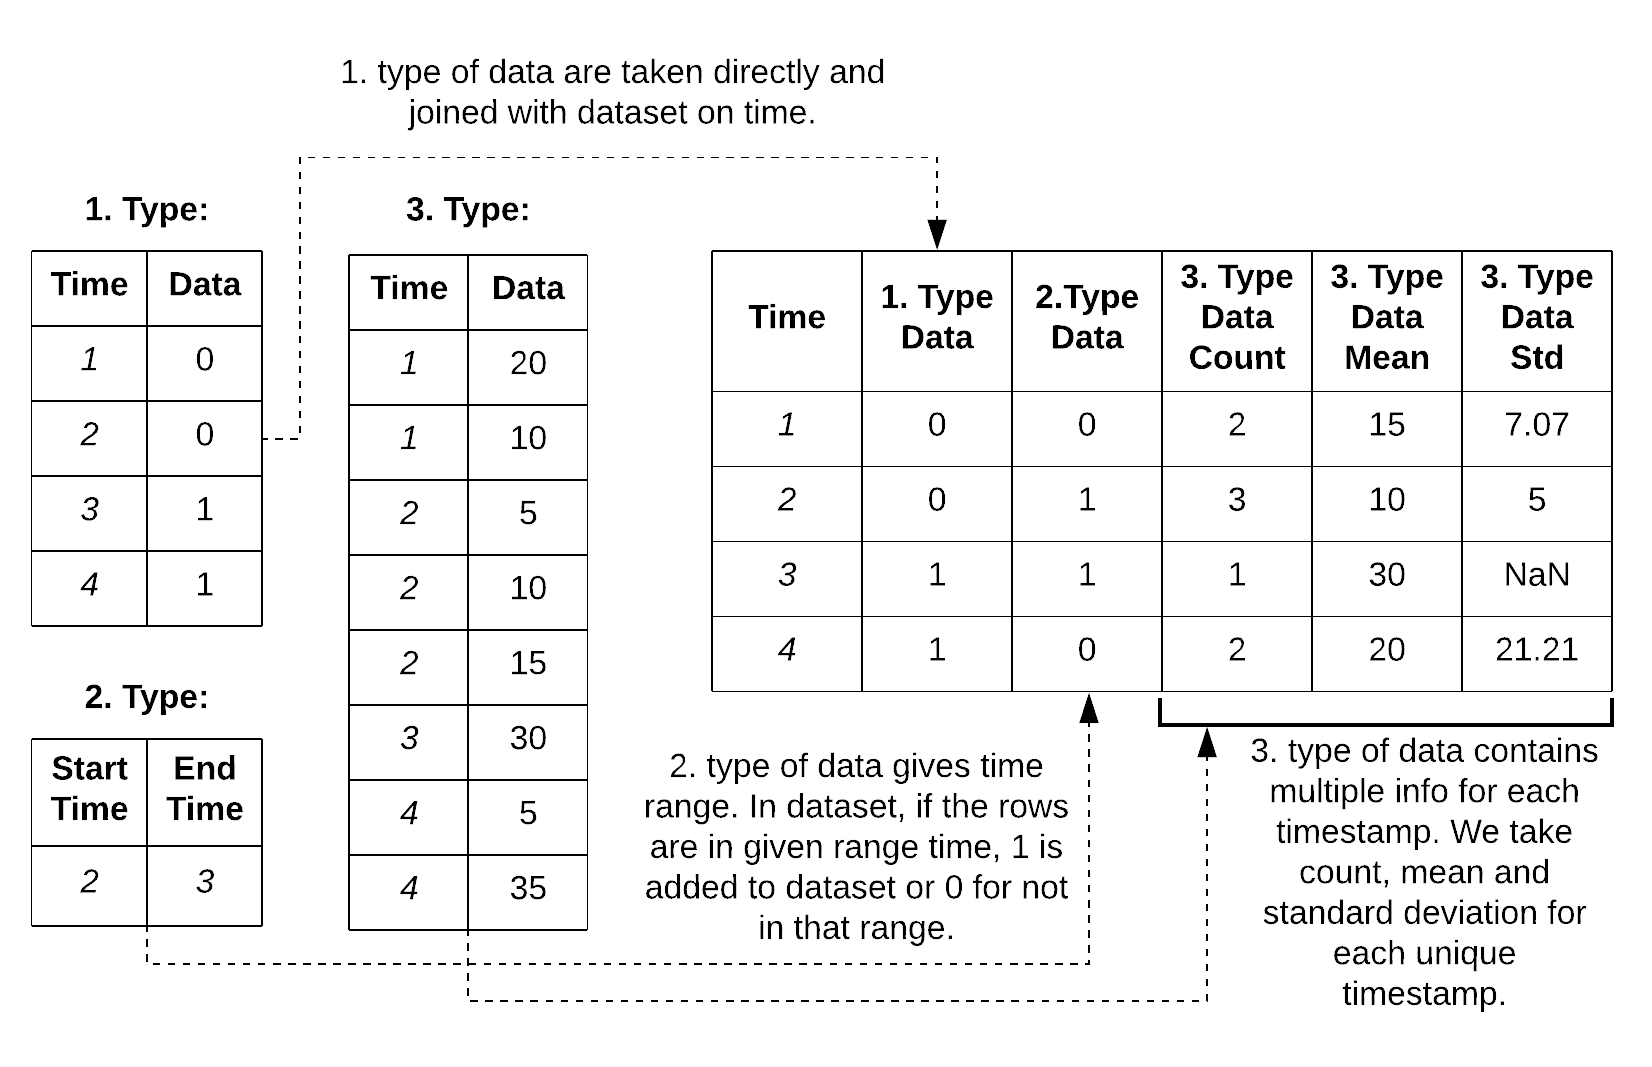
\includegraphics[width=160mm]{graphics/Dataset_Preparation.png}}
\caption{Data Preparation}
\label{fig:Data Prep}
\end{figure}


\begin{figure}[t]\vspace*{4pt}
\centerline{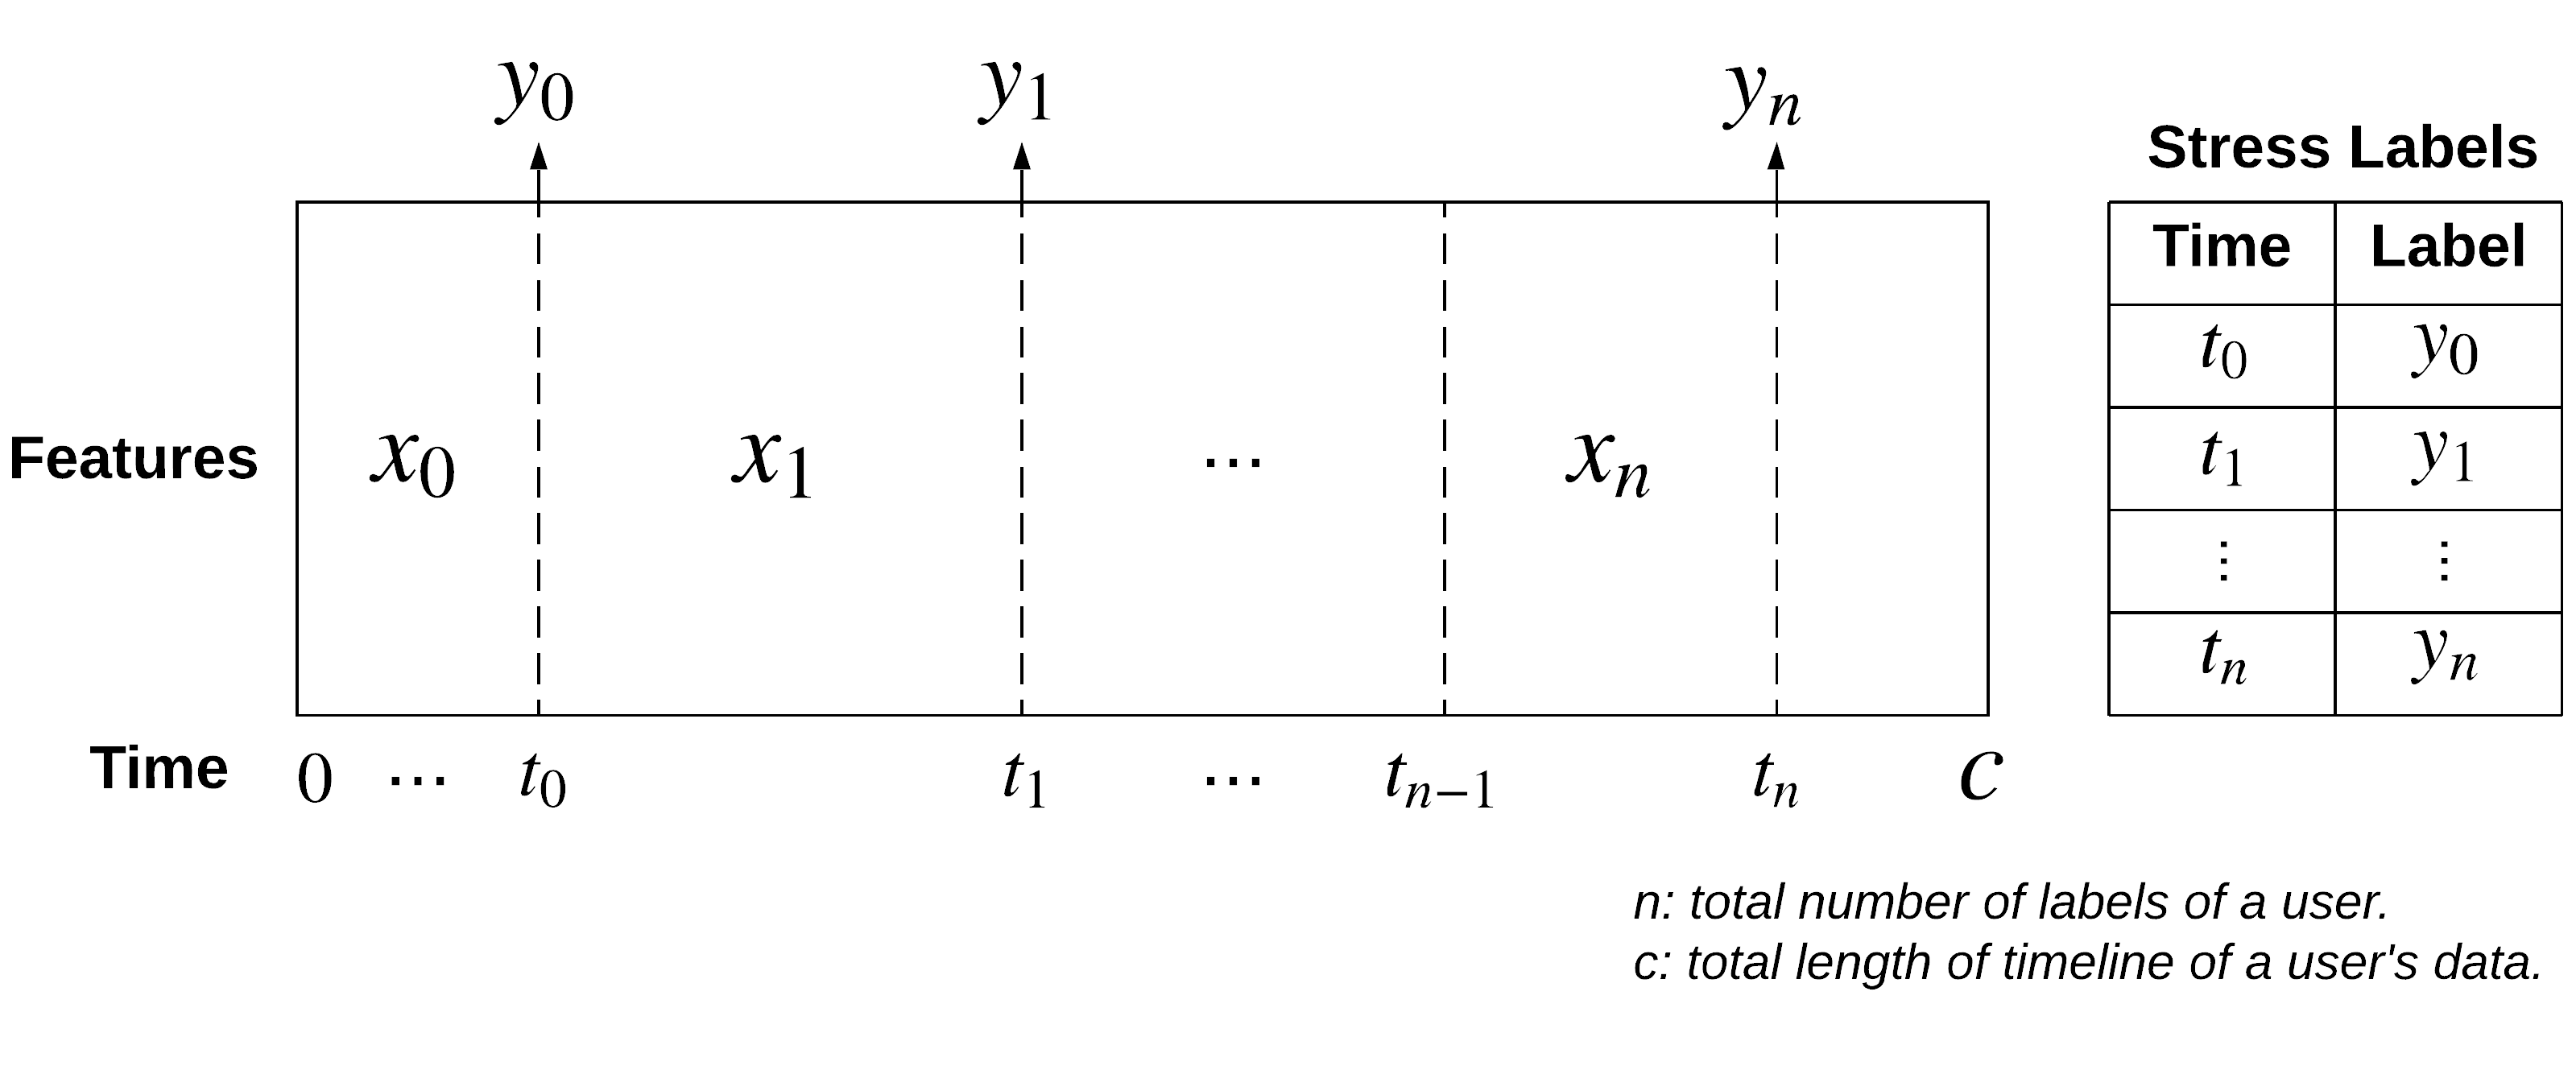
\includegraphics[width=140mm]{graphics/Creating_Instances.png}}
\caption{Instance Creation for RNN}
\label{fig:Instance Creation}
\end{figure}

\subsection{Creating Same Length Instances}
\label{subsec:SameLengthInstances}
Because of the feedback from students can have different time interval, when we extract instances according to stress labels, some instances became too long and some short. We generated the same length instances to feed into the model by padding. If getting feedback from a student took more than 12 hours, we only took the last 12 hours. In similar, if it took less than 12 hours, we added zeros to the forefront of the sequence to create the same sequence as 12 hours. Lastly, if the time interval between two feedback was less than 2 hours, we moved to the next feedback to create an instance. We chose 2-12 hours period because training with very short time interval data which combined with very long time interval can have too many zeros because of padding. 

\subsection{Normalization}
\label{subsec:Normalization}
Data normalization is one of the most utilized data preparation processes in Neural Networks. It makes all input values in a similar range and thus makes the model can learn optimal parameters faster and converges quicker. Moreover, it reduces the probability of getting stuck in the local optima and increase the probability to reach global optima.

We practiced Yeo-Johnson Transformation \cite{yeo2000new}  for data normalization process. It is a more complex calculation than basic normalization/transformation techniques like Min-Max scaling or log transformation but it has some advantages. If the data has non-normal distribution, we can use Box-Cox transformation or Yeo-Johnson transformation to transform data into a normal distribution. However, Yeo-Johnson allows transformation for negative data without worrying about the domain. Yeo-Johnson transformation is defined by

\begin{equation}
\psi(\lambda, y)=\left\{\begin{array}{ll}{\left((y+1)^{\lambda}-1\right) / \lambda} & {\text { if } \lambda \neq 0, y \geq 0} \\ {\log (y+1)} & {\text { if } \lambda=0, y \geq 0} \\ {-\left[(-y+1)^{2-\lambda}-1\right) ] /(2-\lambda)} & {\text { if } \lambda \neq 2, y<0} \\ {-\log (-y+1)} & {\text { if } \lambda=2, y<0}\end{array}\right.
\label{eq:Yeo-Johnson}
\end{equation}

where $ y $  is a list of $ n $ strictly positive numbers, and $\lambda$ includes the important special cases of untransformed, inverse, logarithmic, and square and cube root.

\begin{figure}[t]\vspace*{4pt}
\centerline{
\includegraphics[width=60mm]{graphics/Input_Shape.png}}
\caption{Input Shape}
\label{fig:Input Shape}
\end{figure}

The final format of the data was like in Fig.~\ref{fig:Input Shape}. In there, each instance has a sequence data for each feature and a label for it. For a multi-dimensional array with the shape of (m x s x f), 'm' is the total number of instances, 's' is the sequence length of each instance and 'f' is the total number of features. Additionally, there were labels for each instance in the shape of (m x 1). Lastly, the list of final input features for the model can be seen on Table~\ref{tab:features}.

\begin{table}[b!]
\centering
\caption{List of Features to Feed into Model}
\label{tab:features}
\begin{tabular}{|l|}
\hline
Features                                                       \\ \hline
Activity (Stationary, Walking, Running, Unknown)               \\
Audio (Silence, Voice, Noise, Unknown)                         \\
Is there any conversation?                                     \\
Average signal level to other Bluetooth Devices                \\
Standard deviation of signal levels to other Bluetooth Devices \\
Total number of Bluetooth devices around                       \\
Total number of far Bluetooth devices                          \\
Total number of farther Bluetooth devices                      \\
Total number of near Bluetooth devices                         \\
Total number of nearer Bluetooth devices                       \\
Call log                                                       \\
Total number of deadlines                                      \\
Hour of the day                                                \\
Is the phone charging?                                         \\
Is the phone in the dark?                                      \\
Is the phone locked?                                           \\
Total number of running apps                                   \\
SMS                                                            \\
Average signal level to Wi-Fi spots                            \\
Standard deviation of signal levels to Wi-Fi spots             \\
Total number of Bluetooth devices around                       \\
Total number of far Bluetooth devices                          \\
Total number of near Bluetooth devices                         \\
Total number of nearer Bluetooth devices                       \\ \hline
\end{tabular}
\end{table}


\section{Model Building}
\label{sec:Model Building}
In the model building section we discussed, what type of model we built, which algorithms we chose, why we chose these algorithms, what were the model architectures and which validation tools we utilized.


\subsection{Classification}
\label{subsec:Classification}
Because of our discrete outputs, we need to employ a classification method to reach automatic stress recognition goal. In the classification process, the output label is known and the algorithm tries to separate data into discrete groups. Therefore, we generated 2 classes ("Stressed" and "Not-Stressed") to create a binary classification problem. Label 0 represents "Not-Stressed" and label 1 represents "Stressed" in our task. The percentages for the distributions of the two classes were 68.74\% for "Stressed" and 31.26\% for "Not-Stressed". In general, people expect to have less stressful times and more relaxed times but the distribution was the exact opposite for this dataset. It could be because users may have a tendency to reply to feedback prompts when they were stressed. There are different methods that can be used for classification process and most used ones are Logistic Regression, Nearest Neighbors, Naive Bayes, Support Vector Machines, Decision Trees and Artificial Neural Networks (Multi-Layer Perceptron). These type of methods employed on early works for this subject that we mentioned earlier. However, we would like to try a promising algorithm for sequence data which is Recurrent Neural Network for this classification process. In this work, we utilized Long Short-Term Memory which is a special kind of RNN. Therefore, we prepared our dataset to make it ready to feed as sequence data. To compare results with similar dataset, we chose 2 new and promising algorithms which and CNN (Convolutional Neural Network) and CNN-LSTM (Convolutional Neural Network - Long Short-Term Memory).

\subsection{Long Short-Term Memory}
\label{subsec:LSTM}
For the classification process, the model needs a mapped input instance and an output. The classification methods that were mentioned before RNN need each instance as one shot (fixed-size of a vector). In other words, there is no internal state getting updated in time. Therefore, if there are sequence data, we need to find a way to represent time-varying data in the shape that the model accepts. To decrease the shape of time-series data of an instance, descriptive statistics such as sum, mean, standard deviation, skewness and so forth are usually calculated. Besides, there are some tools for specific domains to represent time-series data in an alternate representation such as Fourier Transformation. However, none of these methods can represent sequence data completely. There is always something missing from the data such as data dependencies.

\begin{figure}[t]\vspace*{4pt}
\centerline{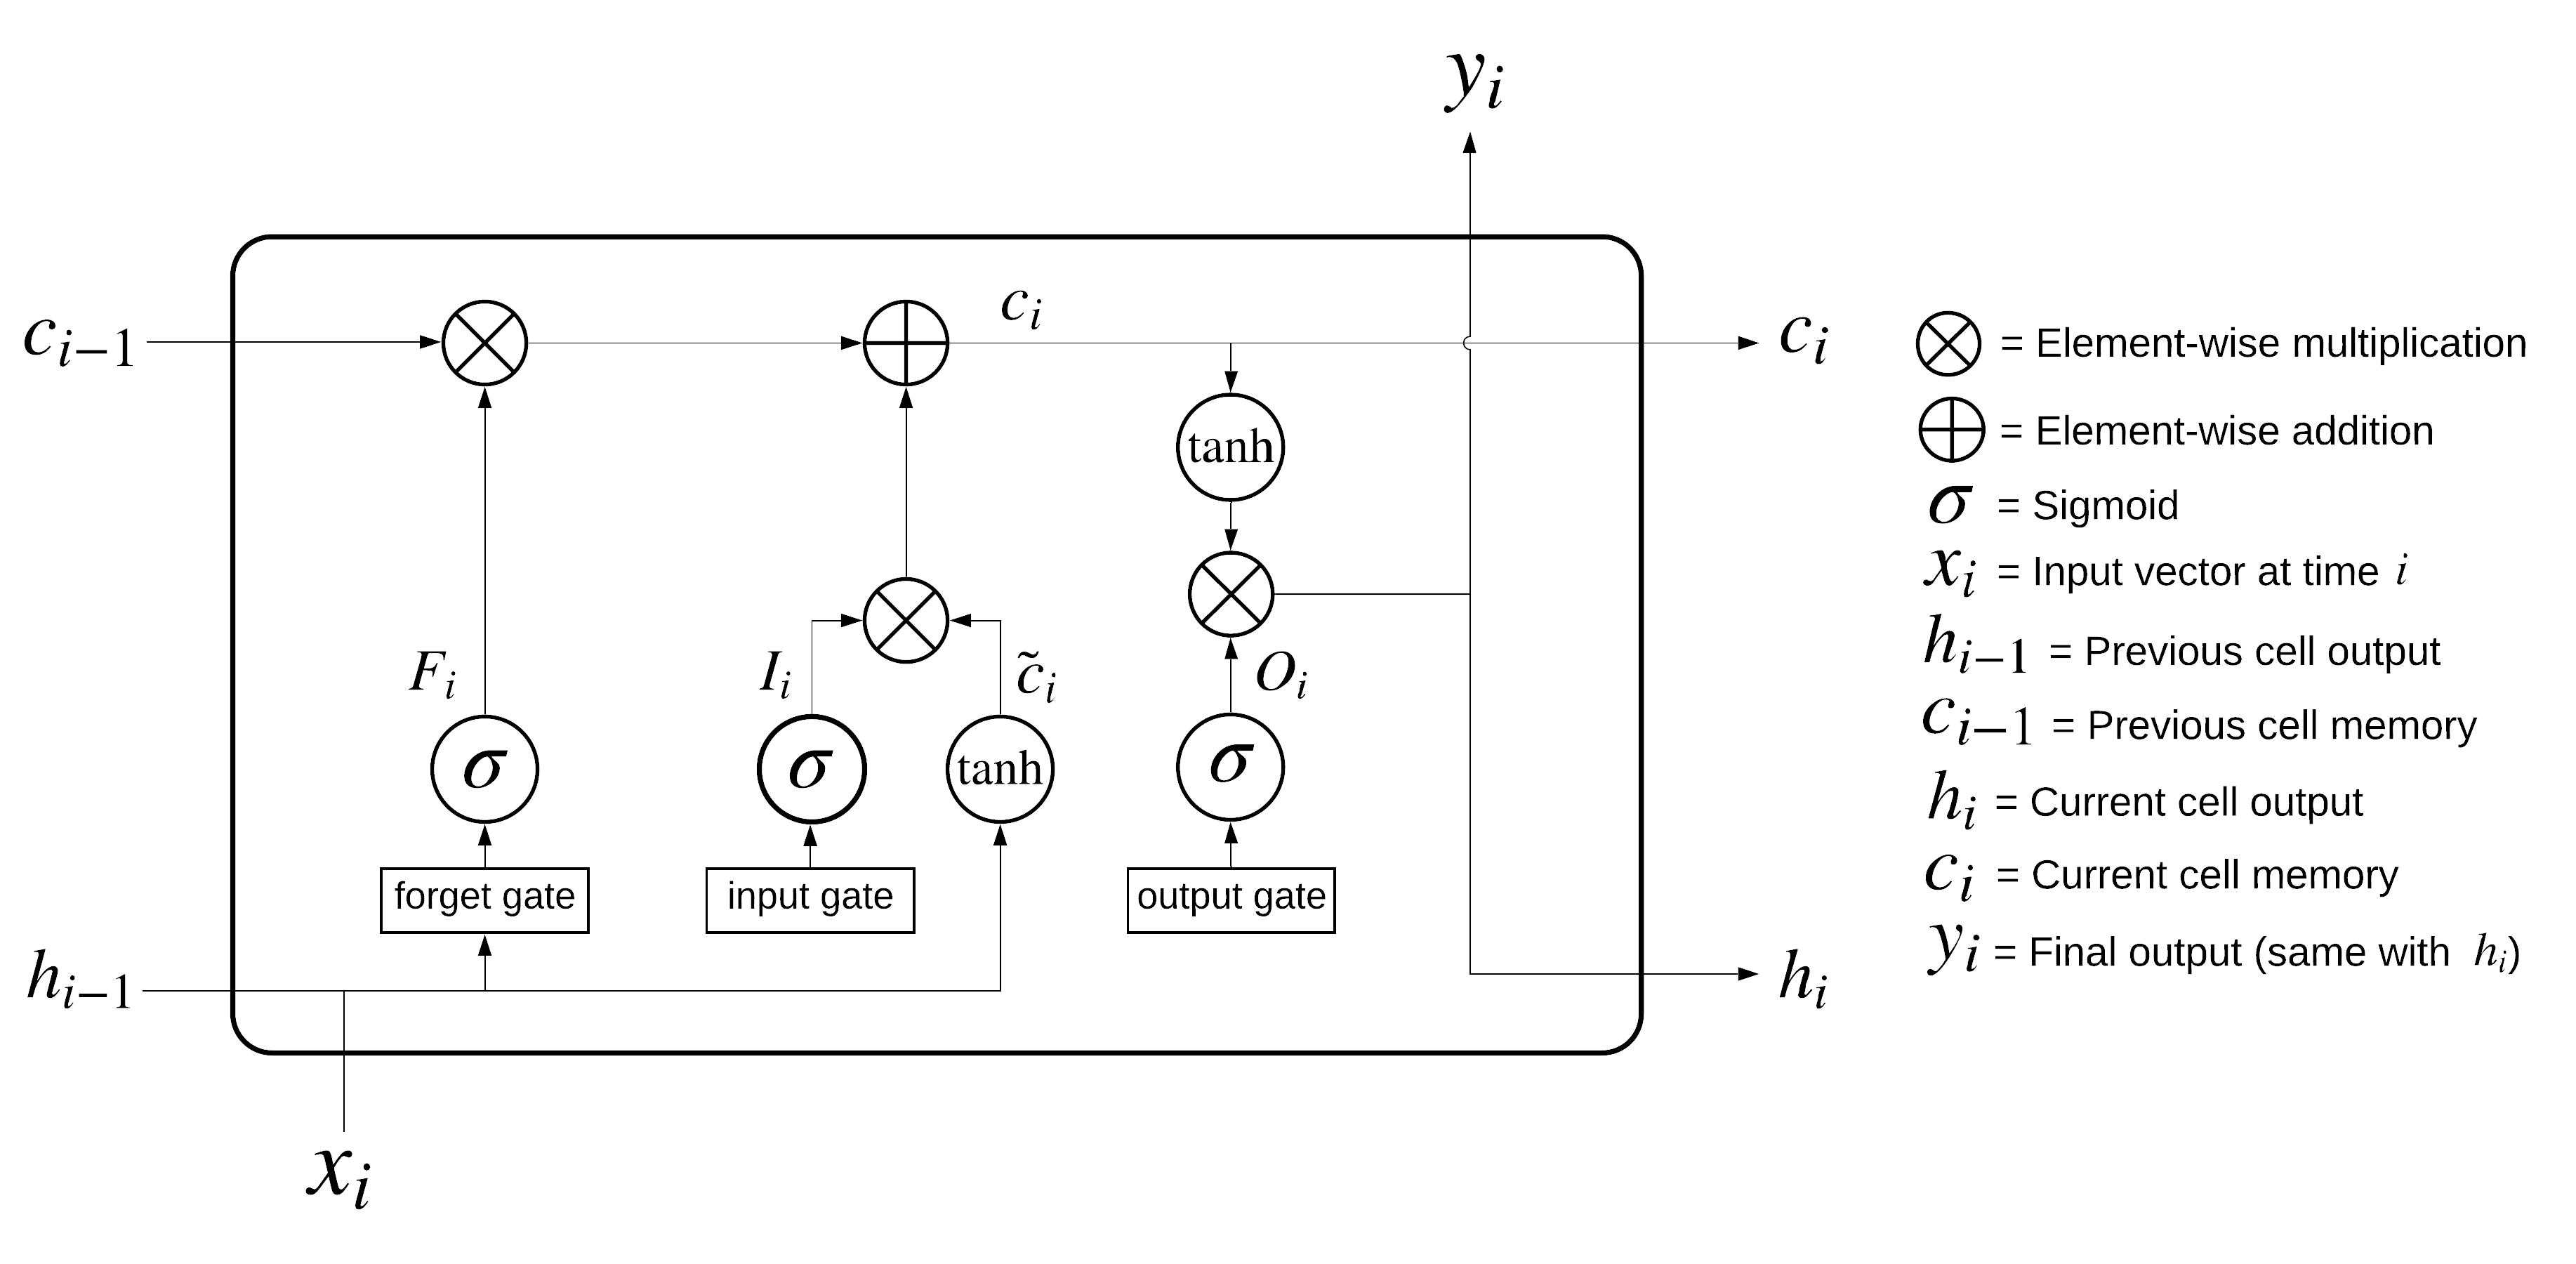
\includegraphics[width=160mm]{graphics/LSTM_Cell.png}}
\caption{LSTM Cell}
\label{fig:LSTM Cell}
\end{figure}

Due to the structure of the Recurrent Neural Network (RNN), we can train a classification model without the preprocessing to decrease the shape of sequence features to one shot vector. RNN models have an internal state which updates in time during model training. Therefore, it can identify the relationships between each sequence to represent the data better. We can think of RNN as multiple copies of a network in a loop and information can pass through a network to another in that loop. Therefore, it can transport data from one step to another in a sequence. Natural language processing (speech recognition, language modeling, translation, etc.) and other types of applications which have sequence data are the areas that utilized RNN to reach exceptional results. Nevertheless, because of the vanishing or exploding gradient problem of RNN, it can only work well on short-term dependencies \cite{bengio1994learning}. Accordingly, Long Short-Term Memory (LSTM) \cite{hochreiter1997long} was emerged to solve this short-term dependency problem and make the network to remember longer dependencies. In addition to RNN structure, LSTM has cell state which transfers the information through each LSTM cell with a minor change in the information. Consequently, the network's default behavior is to remember long-term dependencies. Furthermore, LSTM structure includes three gates (forget gate, update gate, output gate) which decide about the information that goes to the next cell. Forget gate decides what information is eliminated, the input gate selects which values to update and output gate determines what is the output of the cell. An LSTM cell structure and LSTM data workflow can be seen in Fig.~\ref{fig:LSTM Cell} and Fig.~\ref{fig:LSTM Instance}, respectively. Mathematical calculations of LSTM cell is at Equation.~\ref{eq:LSTM} where $F_{i}$ is the forget gate, $I_{i}$ is the input gate and $O_{i}$ is the output gate of the cell. $x_{i}$ is the input values, $W$ with different underscores represent weight matrix of each data and underscore $i$ is for the sequence (time) in the LSTM network. $\tilde{c}_{i}$, $c_{i}$ are the update values for previous cell state and the new cell state, in respectively. $h_{i}$ represents the output of the cell.

\begin{equation}
\begin{array}{l}
{F_{i}=\sigma\left(W_{F}\left[h_{i-1}, x_{i}\right]+b_{F}\right)} \\ {I_{i}=\sigma\left(W_{I}\left[h_{i-1}, x_{i}\right]+b_{I}\right)} \\ 
{\tilde{c}_{i}=\tanh \left(W_{c}\left[h_{i-1}, x_{i}\right]+b_{c}\right)} \\ 
{c_{i}=F_{i} \circ c_{i-1}+I_{i} \circ \tilde{c}_{i}} \\ {O{i}=\sigma\left(W_{O}\left[h_{i-1}, x_{i}\right]+b_{O}\right)} \\ 
{h_{i}=O{i} \circ \tanh \left(c_{i}\right)}\end{array}
\label{eq:LSTM}
\end{equation}

To increase the performance of the LSTM, a lot of model structure and layer combinations have emerged. In this work, we have tried two more models to compare the results of time-series classification. Because of the latest well-performing results in different application, we chose to try Convolutional Neural Networks (CNN) \cite{lecun1995convolutional}. Additionally, the combination of CNN and LSTM \cite{wang2016dimensional} was utilized due to the state-of-the-art results \cite{karim2018lstm}.

\begin{figure}[t]\vspace*{4pt}
\centerline{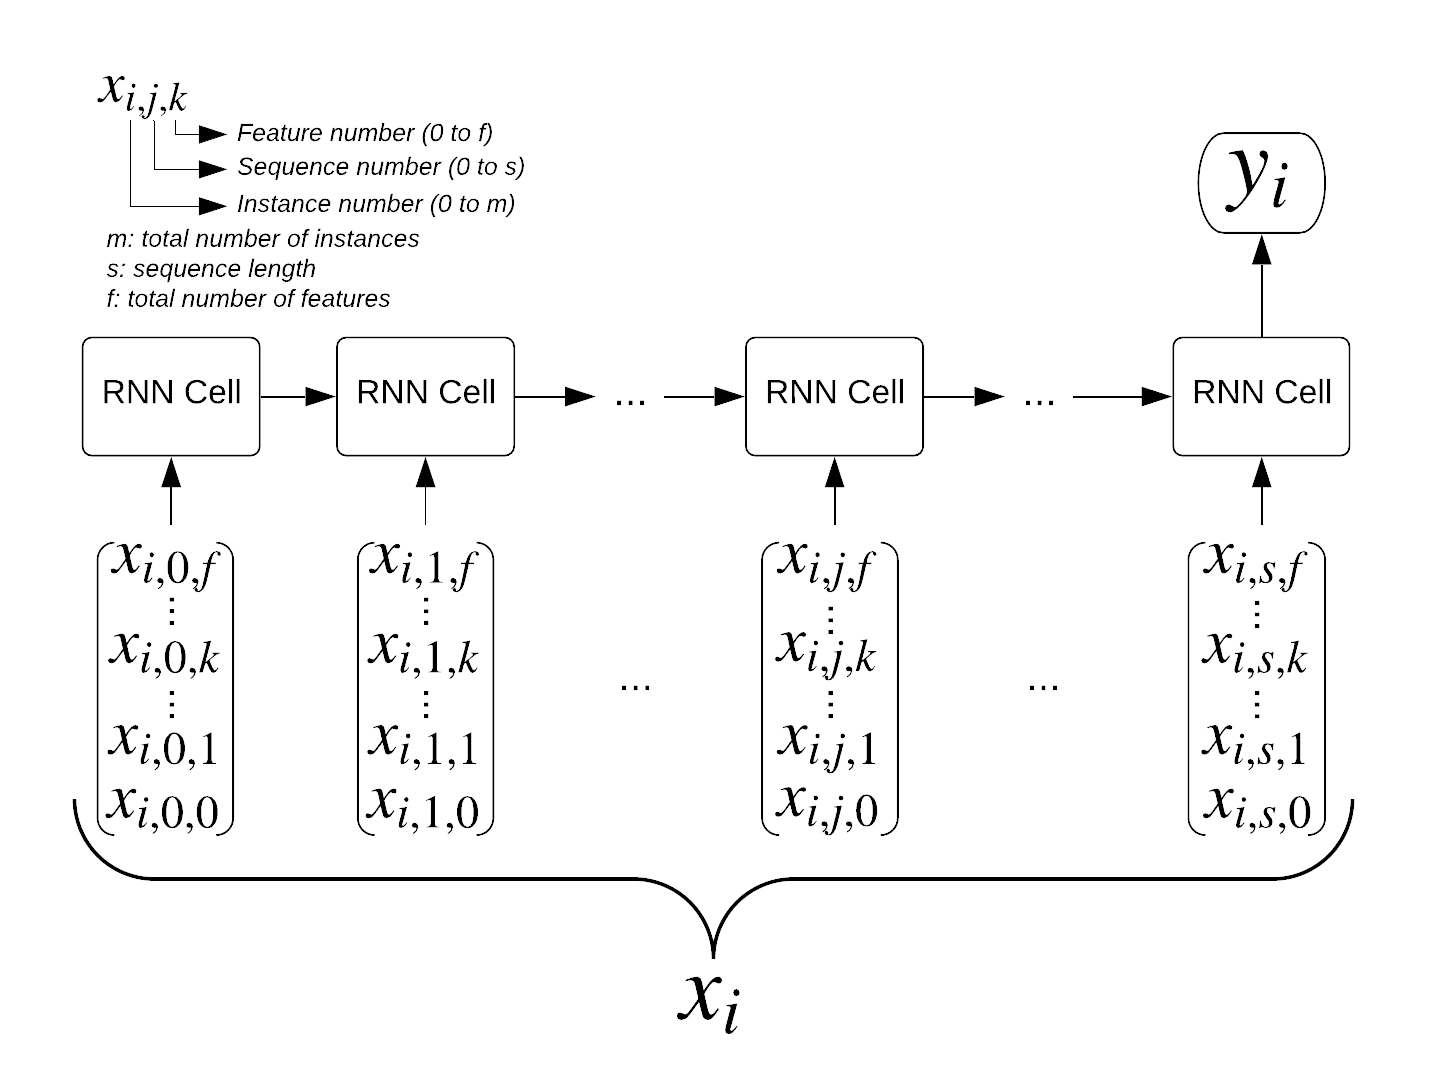
\includegraphics[width=160mm]{graphics/One_LSTM_Instance.png}}
\caption{A LSTM Instance}
\label{fig:LSTM Instance}
\end{figure}

\subsection{Model Architecture}
\label{subsec:Model Architecture}
To reach the best result from the dataset, we tried different model architectures. All the final architectures of LSTM, CNN and CNN-LSTM models can be seen on Fig.~\ref{fig:All Models}. Binary cross-entropy/logarithmic loss and Adam optimizer are used for loss function and optimization in respectively.

\begin{figure}[t]\vspace*{4pt}
\centerline{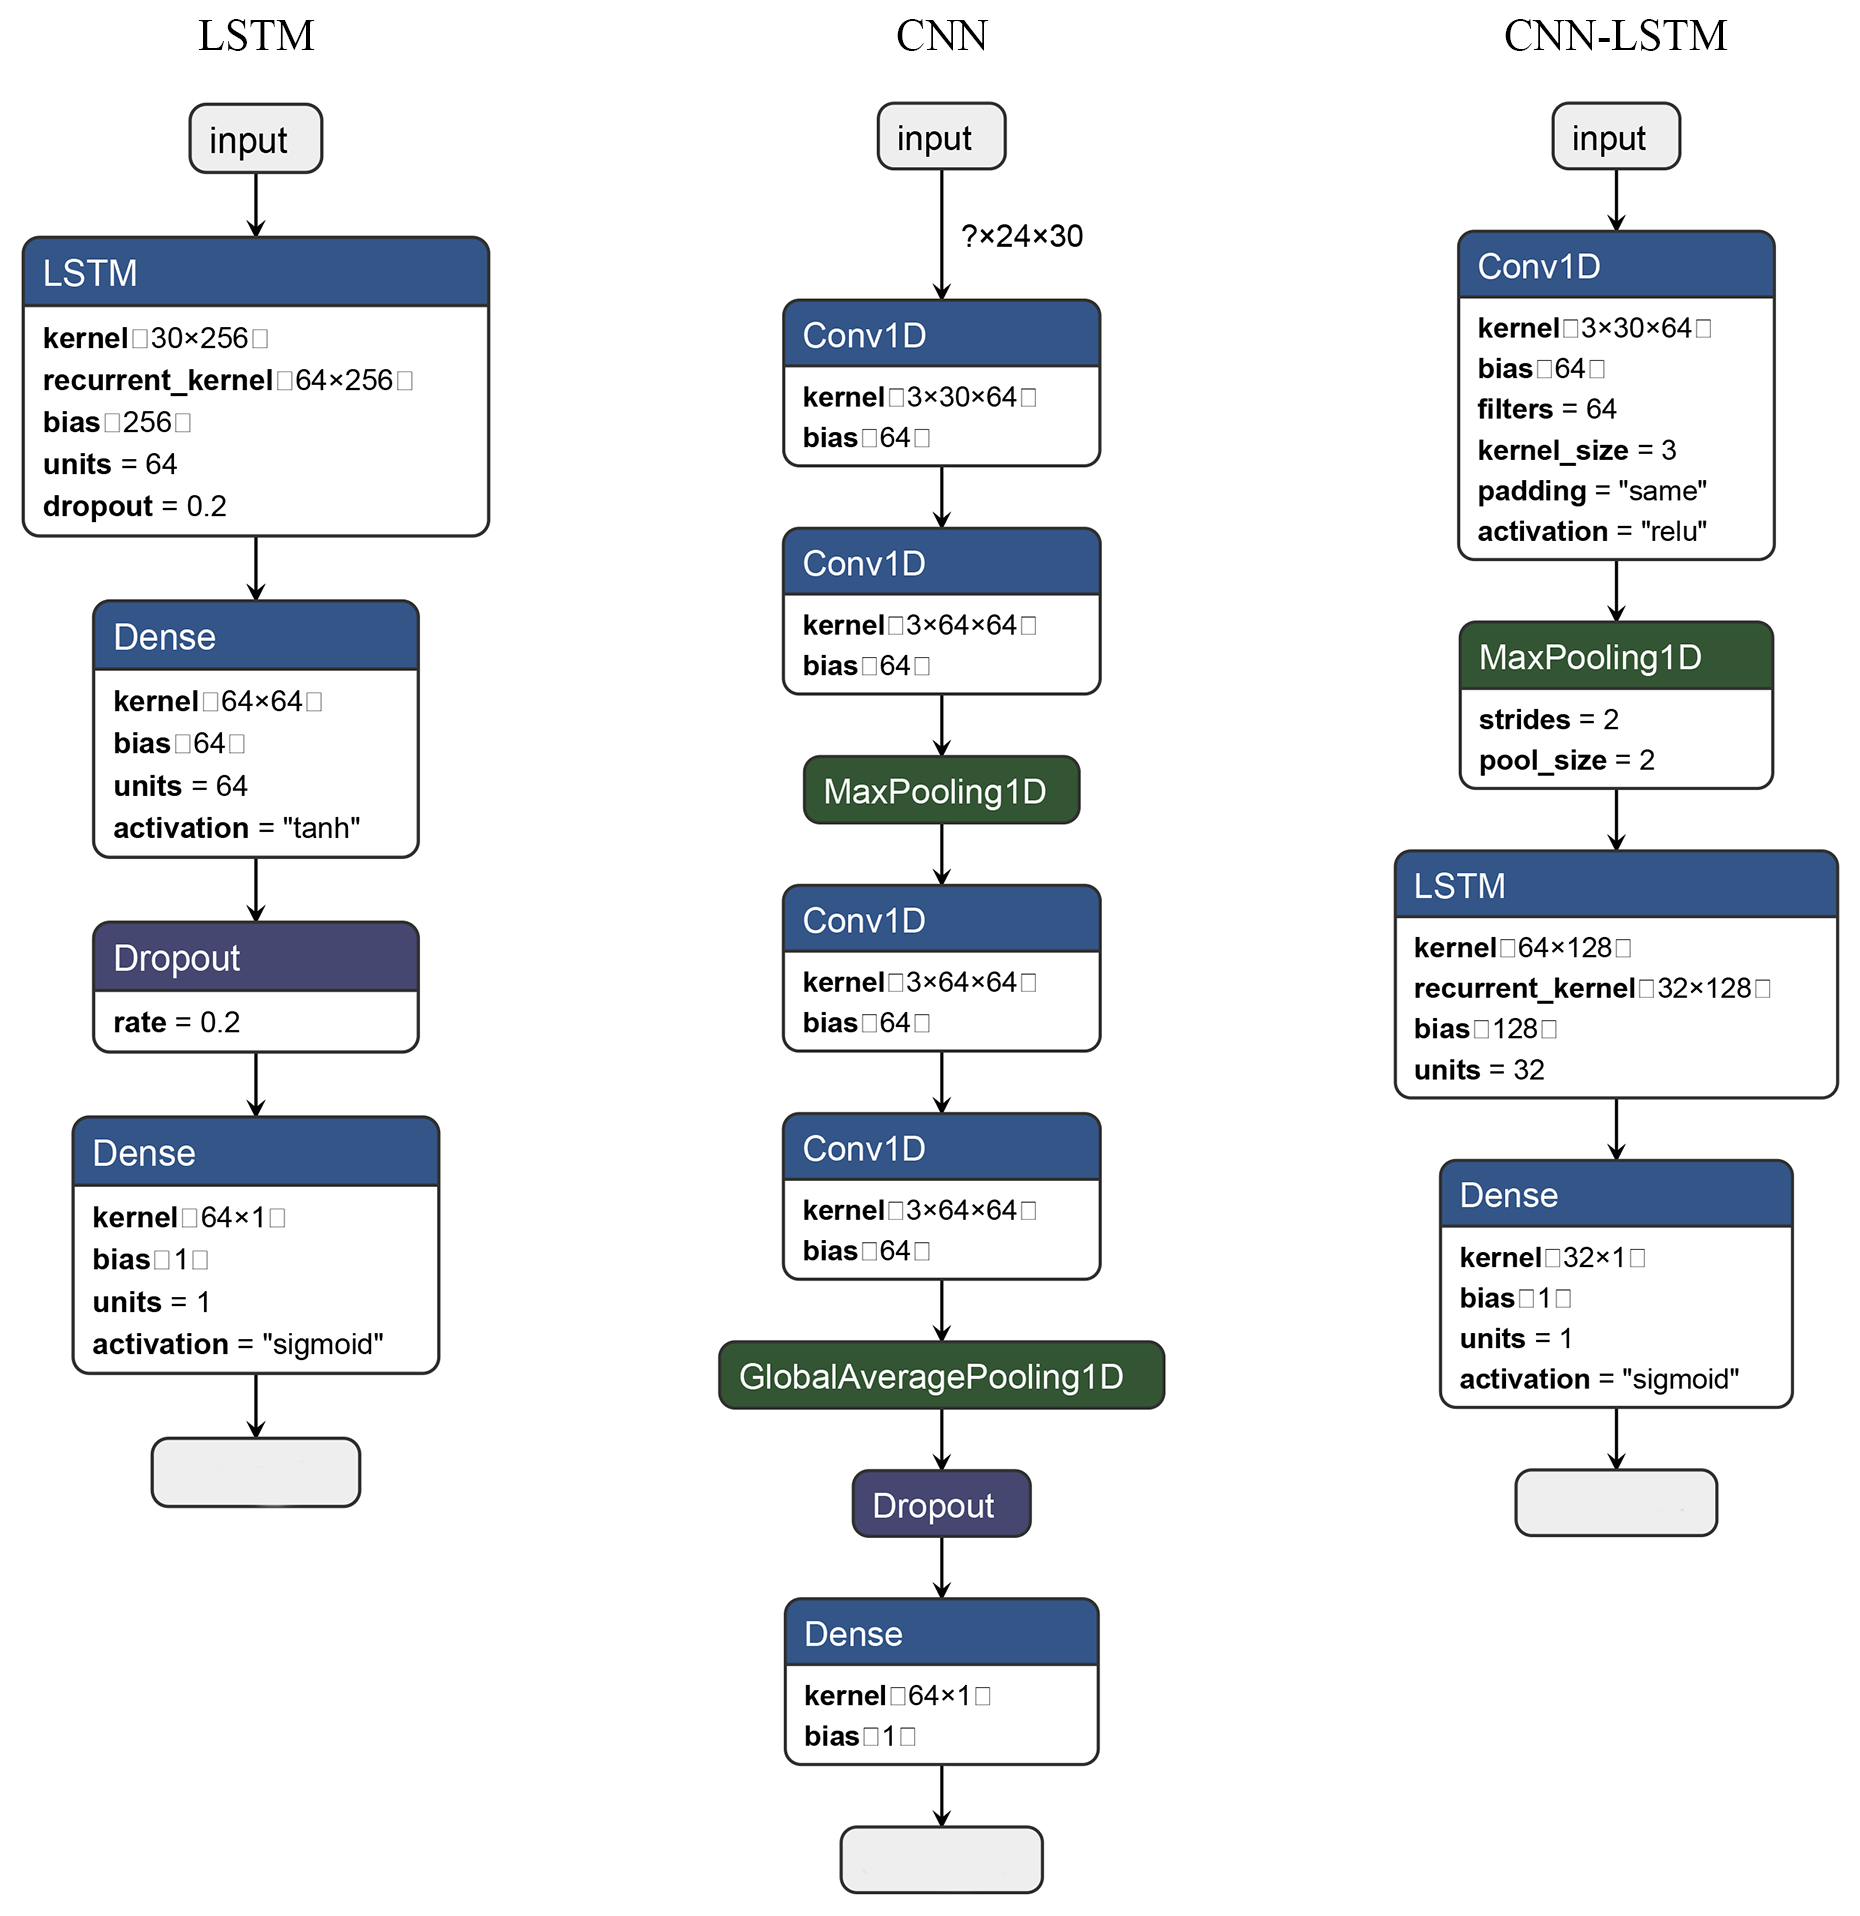
\includegraphics[width=160mm]{graphics/All_model_architectures.png}}
\caption{Model architectures of LSTM, CNN and CNN-LSTM}
\label{fig:All Models}
\end{figure}


\section{Validation}
\label{sec:Validation}

\begin{figure}[t]\vspace*{4pt}
\centerline{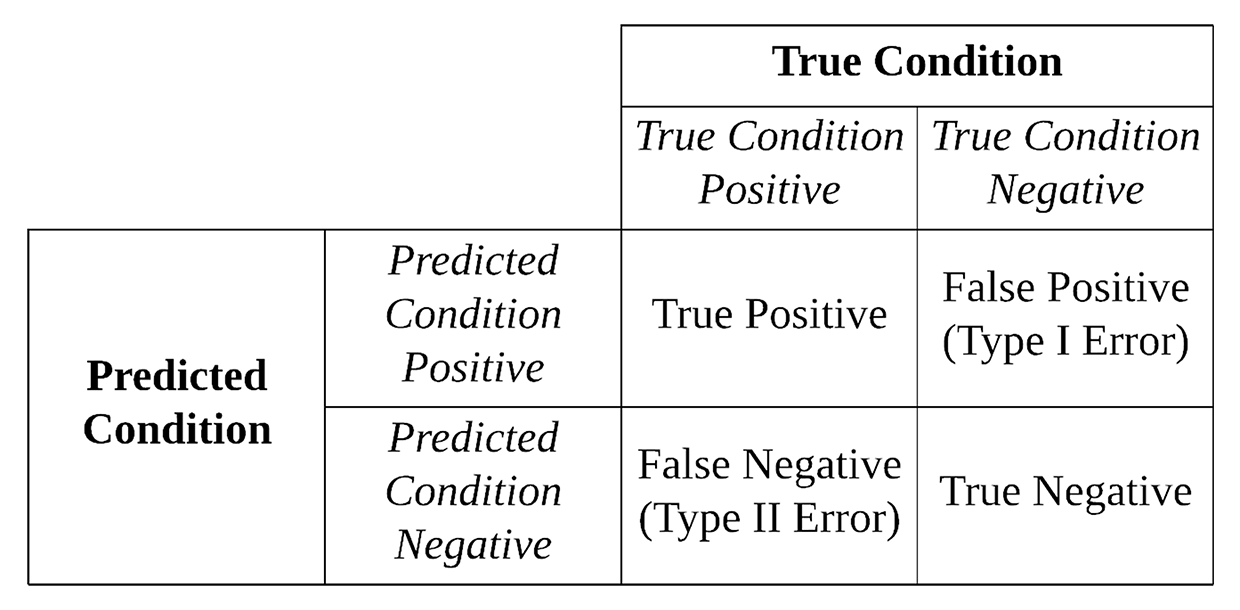
\includegraphics[width=120mm]{graphics/ConfusionMatrix.png}}
\caption{Confusion Matrix}
\label{fig:Confusion Matrix}
\end{figure}

Models should uncover hidden insights from the data without memorizing the training data (overfitting). We utilized different performance metrics to understand the model performance. In classification models, \textit{Accuracy}, \textit{Precision}, \textit{Recall (Sensitivity)}, \textit{F1-Score} and \textit{ROC-AUC} are on the go metrics that decides about the model's performance. Accuracy is the ratio of accurate estimates in the system to all estimates. Precision is a measure of how accurately all classes are predicted. Recall indicates how successful the positive states are predicted. F1-Score is the harmonic average of Recall and Precision. ROC Curve (Receiver Operating Characteristic Curve) \cite{hanley1982meaning} is a graph that represents the classification performance of the model for distinguishing between the True Positives and True Negatives at all classification thresholds. Its axes are True Positive Rate and False Positive Rate. The area under the ROC curve (AUC) is a calculation that measures the performance of the model across all possible thresholds. We calculated these metrics to measure the performance of the model on the test set of our dataset to observe the performance of the model for unseen data. 

Accuracy, Precision, Recall, and F1-Score are calculated from the data that come from the Confusion Matrix. The Confusion matrix shows the prediction results for a classification problem. The correct and incorrect predictions are compared with real values according to the classes. The matrix shows how much the model confused when predicting classes. Confusion matrix has 4 different values which are True Positive,  False Positive, True Negative, False Negative. In True Positive, the real value and prediction are all positive. The real value is negative but the prediction is positive in False Positive. In True Negative, the real value is negative and the model predicts it as a negative. The real value is positive but the model predicts it as a negative in False Negative. From these values, we can calculate our performance metrics for the results of all models. 

\begin{equation}
\text { Precision }=\frac{T P}{T P+F P}
\end{equation}

\begin{equation}
\text { Recall }=\frac{T P}{T P+F N}
\end{equation}

\begin{equation}
\text { Accuracy }=\frac{T P+T N}{T P+T N+F P+F N}
\end{equation}

\begin{equation}
F_{1}=\left(\frac{\mathrm{Recall}^{-1}+\text { Precision }^{-1}}{2}\right)^{-1}=2 \cdot \frac{\text { Precision } \cdot \text { Recall }}{\text { Precision }+\text { Recall }}
\end{equation}


\chapter{Experimental Results}
\label{chap:Experimental Results}
Using continuous passive sensing data of college students, we were able to decide with \%62.83 confidence if the student is stressed or not by looking at their last 2-12 hours mobile sensing data. To train this model, we used 800 training instances, 200 validation instances and 460 test instances, and all of them were balanced dataset. Our sequence length for each instance was 24 and each member of the instance represents 30 min data which means that we look at the data of the student at most 12 hours. 

We aimed to test LSTM because continuous sensor data is time-varying and we thought that the LSTM learning algorithm is very suitable for this dataset. We can feed the time-series data as a sequence to let LSTM discover relationships and dependencies between each time's feature values.

\begin{figure}[t]\vspace*{4pt}
\centerline{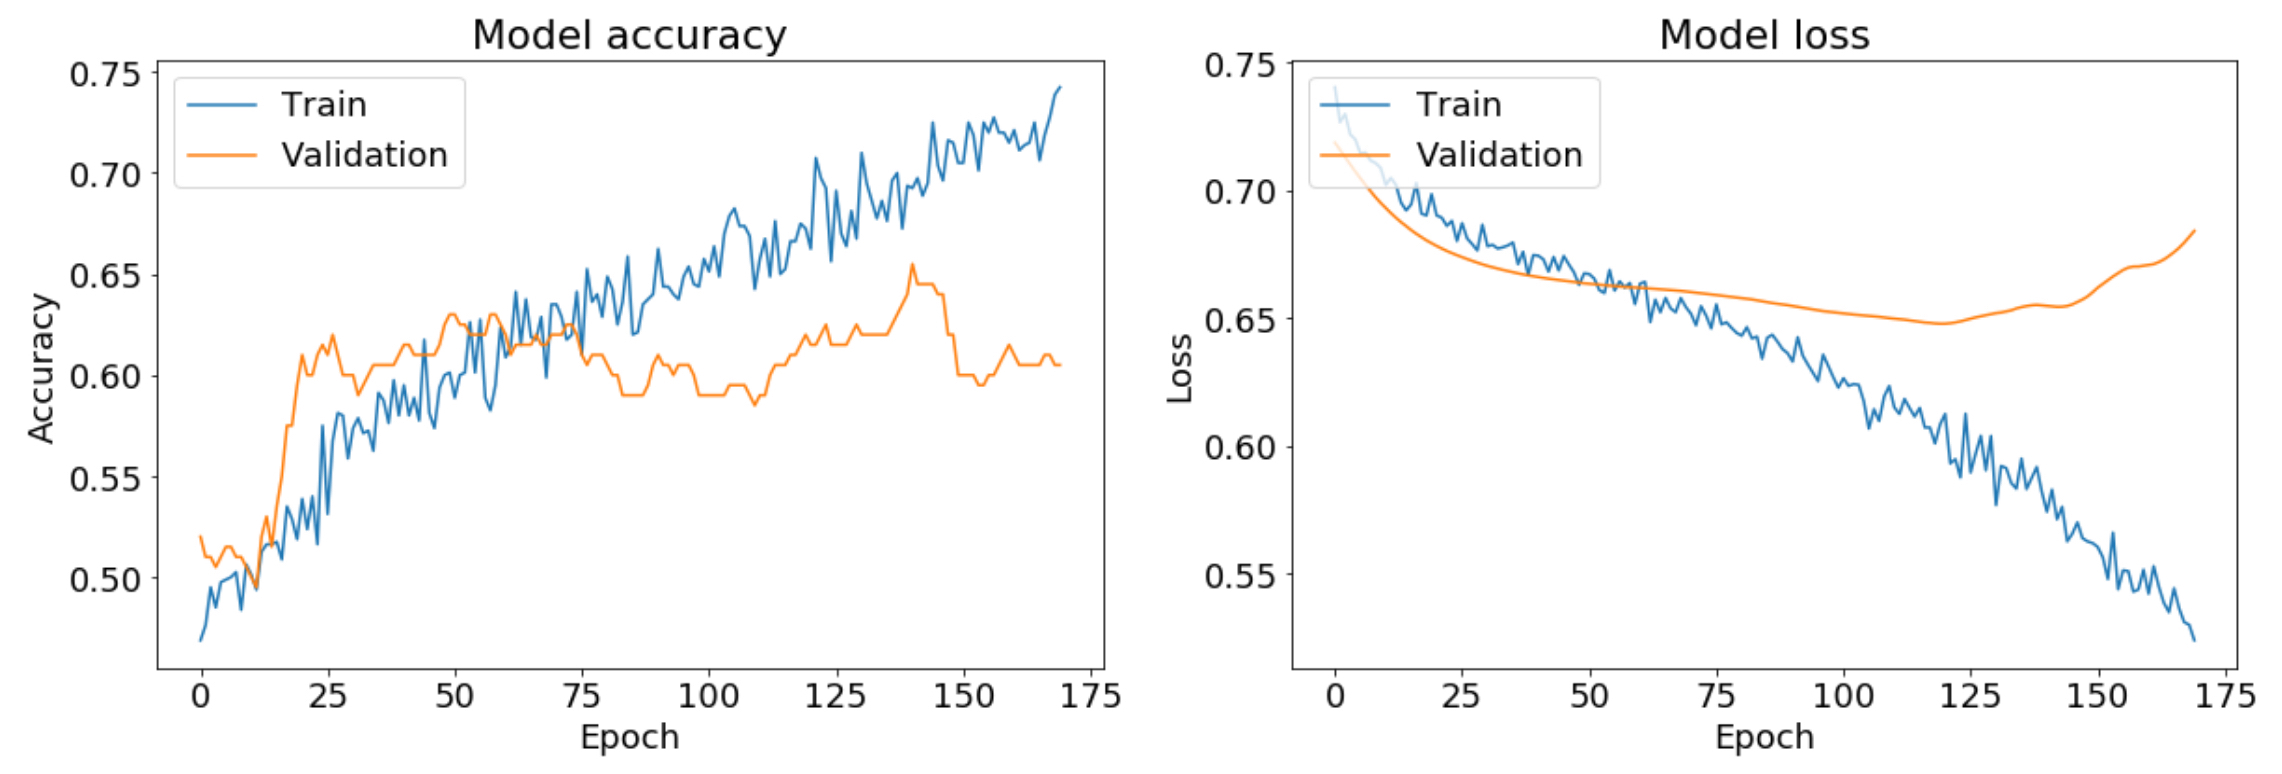
\includegraphics[width=160mm]{graphics/loss_acc.jpg}}
\caption{Accuracy and Loss progress in training}
\label{fig:Accuracy and Loss}
\end{figure}

Accuracy and loss graph of the training process can be seen on Fig.~\ref{fig:Accuracy and Loss}. As we can see that our training and test loss were decreasing until specific epoch and after that point, training loss was decreasing but test loss was increasing. Consequently, we trained our model until that epoch to reach our best generalizable performance. In our tests, if we increase the number of epochs, training performance reaches 100\% accuracy but test performance drops. This is a very clear indicator of overfitting and we tried different methods such as using dropout or decreasing the complexity of the model but none of them helped to solve overfitting problem. We think that this problem occurs because of the data that we have. Adding new features or expanding the size of the data with different samples may help the algorithm to discover more generalizable differences between each class. Precision, Recall, and F1-Score for each class in test data indicate that our model can predict stressed students slightly better which can be seen on Table~\ref{tab:Results}. We trained 3 different models and as it is seen in the Table~\ref{tab:Algorithm Comparison}, all three models' performances were similar to each other but LSTM performs slightly better.

\begin{table}[b!]
\centering
\caption{Model Results}
\label{tab:Results}
\begin{tabular}{|l|l|l|l|l|l|}
\hline
Data         & Accuracy & Precision & Recall & F1-Score & Support \\ \hline
Not Stressed & 0.63     & 0.62      & 0.63   & 0.63     & 230     \\
Stressed     & 0.63     & 0.63      & 0.63   & 0.63     & 230     \\
Average      & 0.63     & 0.63      & 0.63   & 0.63     & 460    
\\ \hline
\end{tabular}
\end{table}


\begin{table}[b!]
\centering
\caption{Comparison of Algorithms}
\label{tab:Algorithm Comparison}
\begin{tabular}{|l|l|l|l|}
\hline
Metric   & LSTM    & CNN     & CNN-LSTM \\ \hline
Accuracy & 62.83\% & 60.43\% & 60\% \\
Precision & 0.63 & 0.6 & 0.6 \\
Recall & 0.63 & 0.6 & 0.6 \\
F1-Score & 0.63 & 0.6 & 0.6 \\ 
\hline
\end{tabular}
\end{table}


\begin{figure}[t]\vspace*{4pt}
\centerline{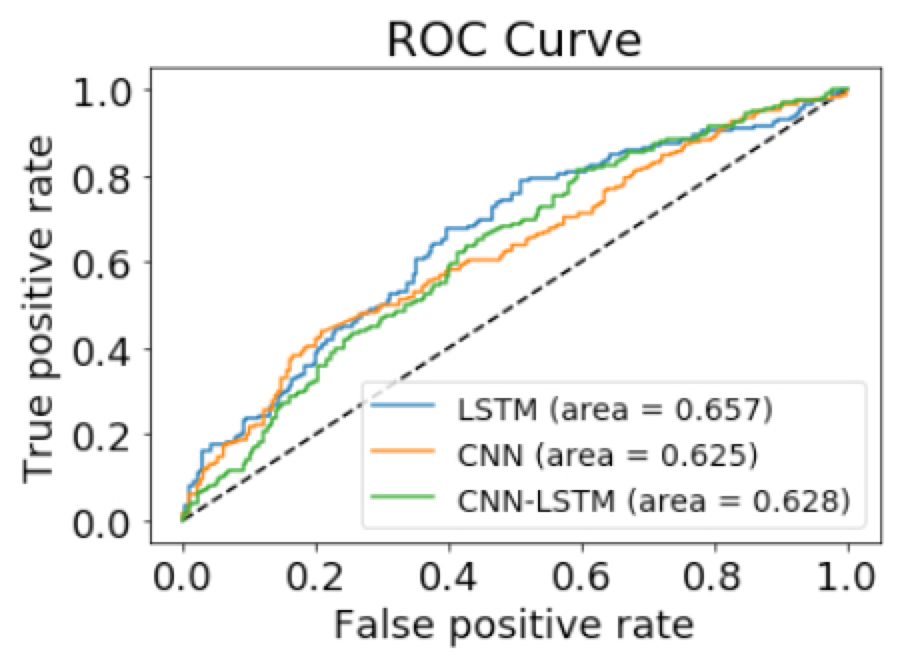
\includegraphics[width=100mm]{graphics/ROC.jpg}}
\caption{ROC Curve of 3 Algorithms}
\label{fig:ROC Curve}
\end{figure}

% REMOVED DATA
%For instance, even if some works could found a relationship between location data and mental health conditions \cite{canzian2015trajectories} we did not use location information because we only have specific locations in the college.

\chapter{Discussion}
\label{chap:Discussion}
Stress is one of the most important problem in our society in last decades.
Continual information retrieval, increased physical and mental workload, pressure on school and work, demanding society and other similar factors conduce stress in daily life. In some examples, when the stress level changes, people can realize the problem and seek help. However, most of the time people have chronic stress but they cannot detect without any help. Even if a little stress helps in the situations that needs increased attention, chronic or high level stress can have several physiological and psychological results as we discussed earlier.   

The ultimate goal to create an human mental health assistant, we implemented the first initiative approach that is automatic stress recognition algorithm. In the final form of the goal, the system will use passive sensor data from mobile phones and daily life wearables such as smart watches, smart glasses, etc. There will be an app which will always run in the background and automatically (without any interaction) detect human emotions (happiness, stress, etc.) during the day. In the end of the day, week and month, the app will create a report of mental health phase changes instead of alerting user with the finding. It will give information about when the user had most stressful or happy moments, and what was s/he doing during these moments. Moreover, it will find relationships between the moments and the emotions for each specific user. Therefore, it would orient people to do thing that will improve their mental health. Online learning will be a part of the system so it will adapt to the user and continually improve as time progresses. Therefore, this technology will prove a cost-effective and reliable tool for human mental health improvement. Even if the system will give report and recommendations to people, the system would be utilized by therapists, psychiatrist, health organizations, etc. 

Stress is a major problem in any environmental condition, but it can have very important personal and crowd-affecting consequences in crowded and interpersonal environments. Therefore, this system can be occupied to detect stress before becoming a bigger problem to support the person. Stress awareness is one of the first steps people should take to avoid stress and prevent stress. As a result, they can reach a healthy mood by taking steps to prevent stress and improve the quality of life and lead to a better life. Most applications developed for stress recognition aim to stimulate people in stressful situations and to offer stress management and relaxation techniques to reduce stress levels. However, we do not think that stimulation will be very successful in stress management because when people are stressed, it is very difficult for people to eliminate it. Instead, a report that summarizes what they do before, when they are not stressed, what they may have been experiencing discomfort, what factors might affect them, what they do when they are not stressed, and what they can do to avoid stress, will do more for people.

In this first step to the final system, our first algorithm detects daily stress with an accuracy of 62.83\% combining passive sensor data and logs from mobile phones. Creating a stress recognition system was the first but essential step because the ultimate system cannot be done without recognizing the stress. The works that were done previously in similar datasets does not show very accurate results for predictive models \cite{wang2014studentlife, dasilva2019correlates, becker2016predict, pratap2019accuracy}. However, they have found that there are relationships between mobile passive sensing data and stress. They were also showed that user based models outperform general models in prediction performance. Nevertheless, we created a general model which means that the results are not for a specific student, they are valid for all students. In that case, the algorithm should find general pattern between each stressful and not stressful student so it is a harder task than user specific developments and needs more data to uncover hidden common relationships between stress and passive sensor data.

Because we are trying to make a general model in our work, we did not use any data that cannot generalize well on every condition. When the new data will be collected to create more diversity in the dataset, we can insert to improve the performance of the model. Our ultimate objective is to predict stress and orient people to have a less stressful life. There were studies that we discussed earlier were also trying to predict a person's mood or stress with different algorithms; however, we tried one of the most successful algorithms (LSTM) for time-series data in latest years to improve the performance. Even if the algorithm gave great promises for time-series application at first, our features and sample size cannot generate great results but encourage us to improve the dataset and features to reach our goal.

The limitations encountered in reaching very good performance from the developed algorithm and the steps that can be taken to develop a better and more applicable model should be addressed in order to create a successful automatic human mental health assistant. Here is the outline of some key aspects that influence the model performance.

\begin{itemize}
  \item The dataset that we used in this work is publicly available dataset and there are some problems with data quality. Because of we cannot reach the raw data, we need to use some labeled data to train our model that may decrease our performance.
  \item Our dataset contains a lot of discrete data. However, Neural Network architectures perform better with continuous data. Therefore, the performance of the model can be related to data type.
  \item Our sample comes from a college student population who spent most of their times in college campus. Therefore, they do not represent whole population and the results could be highly biased to specific type of people.
  \item The data used only comes from people who have collected data. We do not have enough access to social interactions because there is not enough data from people around them.
  \item The performance of the model can be improved with data from a variety of sources. Some studies have tried to improve the performance of the model by adding attributes such as weather. By adding different attributes like this, the model can be enabled to find links between them.
  \item The diversity of data from the social life of people can be increased. For example, there may be a lot of people around the user, but these people can be friends at work. Instead, they can be happier when they spend time with their families with less people.
  \item The data used is the biggest problem experienced in the desired model to be developed. Algorithms that require high amounts of data, such as RNN, find it difficult to generalize when they cannot see a sufficient variety of samples. This LSTM model, which has been trained with 800 samples, does not perform very well, but it motivates us to collect more data.
\end{itemize}

Accordingly, we aim to collect more data in the following works to increase the size of our dataset, so we can compare user-specific models and general models. Additionally, more data may improve our results from 62.83\% accuracy for the general model. 


\chapter{Conclusion and Future Work}
\label{chap:Conclusion and Future Work}
In this work, we created a model to predict the stress levels of students for the purpose of our ultimate goal which is a system that analyses human previous passive data and makes predictions about mental health conditions and give insights about findings to users. We used StudentLife dataset which has mobile sensing and stress feedback data from college students. The data was preprocessed to make it ready for RNN algorithm structure. Specifically, LSTM algorithm was adopted to classify stressed and not stressed students with time-series features. The accuracy of the model on the balanced test set is 62.83\%. Further research will be directed to include more diverse data from people from different background and to increase feature size to improve the model's performance. Furthermore, after creating a base model which has a satisfactory results, we want to adopt the online learning technique to make the model adapt to the user with new data. In the end, it is aimed that there will be an automatic human mental health assistant which always controls mental state in the background, and give a report and mental health improvement methods.


\bibliography{thesis_references}
\bibliographystyle{dcu}

\curriculumvitae
Yasin Açıkmeşe was born in Mannheim/Germany on June 26, 1990. He studied at Kenan Evren Anatolian High School where he was graduated in 2008. He attended the undergraduate program of Manufacturing Systems/Industrial Engineering at Sabancı University. He received his B.S. degree in the Manufacturing Systems/Industrial Engineering in 2013. He worked at Akbank, Golive Consulting and Inovatink in the early years of the professional career. Now, he works at Tekkredi as a Data Scientist since October 2018 and continues to work towards a master’s degree in Logistics and Financial Management under the supervision of Assoc. Prof. Dr. Sadettin Emre Alptekin the Institute of Science and Engineering, Galatasaray University.

The papers that have appeared as full text in refereed proceedings of international conferences:

Acikmese, Y., Ustundag, B. C., & Golubovic, E. (2017, November). Towards an artificial training expert system for basketball. In 2017 10th International Conference on Electrical and Electronics Engineering (ELECO) (pp. 1300-1304). IEEE.

Uzunovic, T., Golubovic, E., Tucakovic, Z., Acikmese, Y., & Sabanovic, A. (2018, October). Task-Based Control and Human Activity Recognition for Human-Robot Collaboration. In IECON 2018-44th Annual Conference of the IEEE Industrial Electronics Society (pp. 5110-5115). IEEE.

The papers that accepted as full text in refereed proceedings of international conferences:

Acikmese, Y., Alptekin, S. E. (In Proceeding). Prediction of stress levels with LSTM and passive mobile sensors. In 2019 23rd International Conference on Knowledge-Based and Intelligent Information & Engineering
Systems (KES).

\label{chapter:vita}
\thispagestyle{empty}

\end{document} 